\documentclass[12pt]{article}
\usepackage{graphicx}
\usepackage{setspace}
\usepackage{fancyhdr}
\usepackage{amssymb}
\usepackage{xcolor}
\usepackage{amsmath}
\usepackage{svg}
\usepackage{hyperref}
\usepackage{graphicx}
\usepackage{makecell}
\usepackage[a4paper, margin=1in]{geometry}
\pagestyle{fancy}
\lhead{Spherical Spline Implementation}
\rhead{Aliakbar Zarkoob}

\begin{document}
	
	\begin{titlepage}
		\begin{center}
			
			
\includegraphics[height=4cm]{University_of_Tehran_Transparent_BW_logo.png} \hfill
			
\includegraphics[height=4cm]{Fanni_Alt_BW_Logo.png}
			
			\vspace{1cm}
			
			\Large \textbf{School of Surveying and Geospatial Engineering}\\
			\large {Department of Geodesy and Hydrography}
			
			\vspace{3cm}
			
			\huge \textbf{Spherical Spline Implementation}
			
			\vspace{3cm}
			
			\Large \textbf{Author:}\\
			\Large Aliakbar Zarkoob
			
			\vspace{2cm}
			
			\Large \textbf{Professor:}\\
			Dr. Abdolreza Safari
			
			\vfill
			
			\large {Winter 2025}
			
		\end{center}
	\end{titlepage}
	
	
	\section{Introduction}
	
	Spherical spline interpolation has emerged as a critical tool in addressing approximation problems on the sphere, particularly in fields such as geophysics, physical geodesy, and environmental sciences. The increasing availability of high-resolution, spatially distributed data, such as those generated by satellite-based techniques, has necessitated the development of robust mathematical methods to approximate functions defined on spherical domains. Such functions often represent physical quantities like temperature, pressure, ozone concentration, gravitational and magnetic forces, or elastic deformation. These quantities are typically sampled at discrete, irregularly spaced points on the Earth's surface, requiring interpolation methods that can accurately reconstruct them over the entire spherical domain.
	
	Traditional Euclidean methods for localized approximation are often inadequate for global problems on the sphere, such as gravity field determination. The fundamental challenge lies in the lack of a differential mapping that can transform the entire sphere into a bounded planar region without distortion. This limitation has driven the development of approximation methods specifically tailored to spherical domains. Among these, spherical spline interpolation stands out for its ability to model global phenomena effectively while maintaining desirable mathematical properties, such as smoothness and stability.
	
	This report is focused on spherical spline interpolation for gravity potential data, where three distinct kernels (Abel-Poisson, Singularity, and Logarithmic) are employed for interpolating data from a global 6-degree regular grid to a finer 3-degree grid.
		
	\section{Implementation Steps}
	
	The answer for spherical spline is linear combination of the kernel function, as shown in the equation \ref{eq:spherical_spline_ans}. Where $y$ is a desired point, $x_i$ are the input points, $a_i$ are the coefficients for spherical spline interpolation, and $N$ is the number of input points.
	
	\begin{equation}
		S(y) = \sum_{i=1}^{N}a_iK(x_i,y)
		\label{eq:spherical_spline_ans}
	\end{equation}
	
	The coefficients can be calculated from the linear system of equations shown in equation \ref{eq:cal_coeff}. The matrix equation is shown in equation \ref{eq:cal_coeff_matrix}. Where both $x_i$ and $y_i$ represent input points and $F(y_j)$ are the values at input points. Thus the coefficients can be calculated by inverting the design matrix ($A$).
	
	\begin{equation}
		F(y_j) = \sum_{i=1}^{N}a_iK(x_i,y_j) \;\;,\;\; j=1,2,\dots,N
		\label{eq:cal_coeff}
	\end{equation}
	
	\begin{equation}
		\begin{bmatrix}
			F(y_1) \\ F(y_2) \\ \vdots \\ F(y_N) 
		\end{bmatrix}
		= 
		\begin{bmatrix}
			K(x_1,y_1) & K(x_2,y_1) & \dots & K(x_N,y_1) \\
			K(x_1,y_2) & K(x_2,y_2) & \dots & K(x_N,y_2) \\
			\vdots & \vdots & \ddots & \vdots \\
			K(x_1,y_N) & K(x_2,y_N) & \dots & K(x_N,y_N) \\
		\end{bmatrix}
		\begin{bmatrix}
			a_1 \\ a_2 \\ \vdots \\ a_N
		\end{bmatrix}
		\equiv l = Ax
		\label{eq:cal_coeff_matrix}
	\end{equation}
	
	\begin{equation}
		\hat{x}=A^{-1}l
	\end{equation}
	
	After the coefficients are calculated, the value at any desired point can be calculated from the equation \ref{eq:spherical_spline_ans}, or the matrix equation of \ref{eq:spherical_spline_ans_matrix} for $U$ Points.
	
	\begin{equation}
		\begin{bmatrix}
			S(y_1) \\ S(y_2) \\ \vdots \\ S(y_U) 
		\end{bmatrix}
		= 
		\begin{bmatrix}
			K(x_1,y_1) & K(x_2,y_1) & \dots & K(x_N,y_1) \\
			K(x_1,y_2) & K(x_2,y_2) & \dots & K(x_N,y_2) \\
			\vdots & \vdots & \ddots & \vdots \\
			K(x_2,y_U) & K(x_2,y_U) & \dots & K(x_N,y_U) \\
		\end{bmatrix}
		\begin{bmatrix}
			a_1 \\ a_2 \\ \vdots \\ a_N
		\end{bmatrix}
		\label{eq:spherical_spline_ans_matrix}
	\end{equation}
	
	As mentioned, three kernel functions of Abel-Poisson, Singularity, and Logarithmic are used in this project. These three functions are defined in the equations \ref{eq:abel_possion} to \ref{eq:logarithmic}. Where $x$ and $y$ are Cartesian coordinate vectors of a point on the sphere, and $h$ is the smoothing parameter of the kernel which it's value is in range of $(0,1)$.
	
	\begin{equation}
		K_{Abel-Poisson}(x,y) = \frac{1}{4\pi} \frac{1-h^2}{(L_h(x,y))^{\frac{3}{2}}}
		\label{eq:abel_possion}
	\end{equation}

	\begin{equation}
		K_{Singularity}(x,y) = \frac{1}{2\pi} \frac{1}{(L_h(x,y))^{\frac{1}{2}}}
		\label{eq:singularity}
	\end{equation}
	
	\begin{equation}
		K_{Logarithmic}(x,y) = \frac{1}{2\pi h} \ln \left(1 +  \frac{2h}{(L_h(x,y))^{\frac{1}{2}} + 1 - h} \right)
		\label{eq:logarithmic}
	\end{equation}
	
	\begin{equation}
		L_h(x,y) = 1 + h^2 - 2h\left<x,y\right>
	\end{equation}
	
	As mentioned before, data used in this project is gravity potential. This data was acquired from ICGEM \footnote{International Center for Global Earth Models: \url{https://icgem.gfz-potsdam.de}}, and it's shown in the figure \ref{fig:MainData}.

	\begin{figure}[h!]
		\centering
		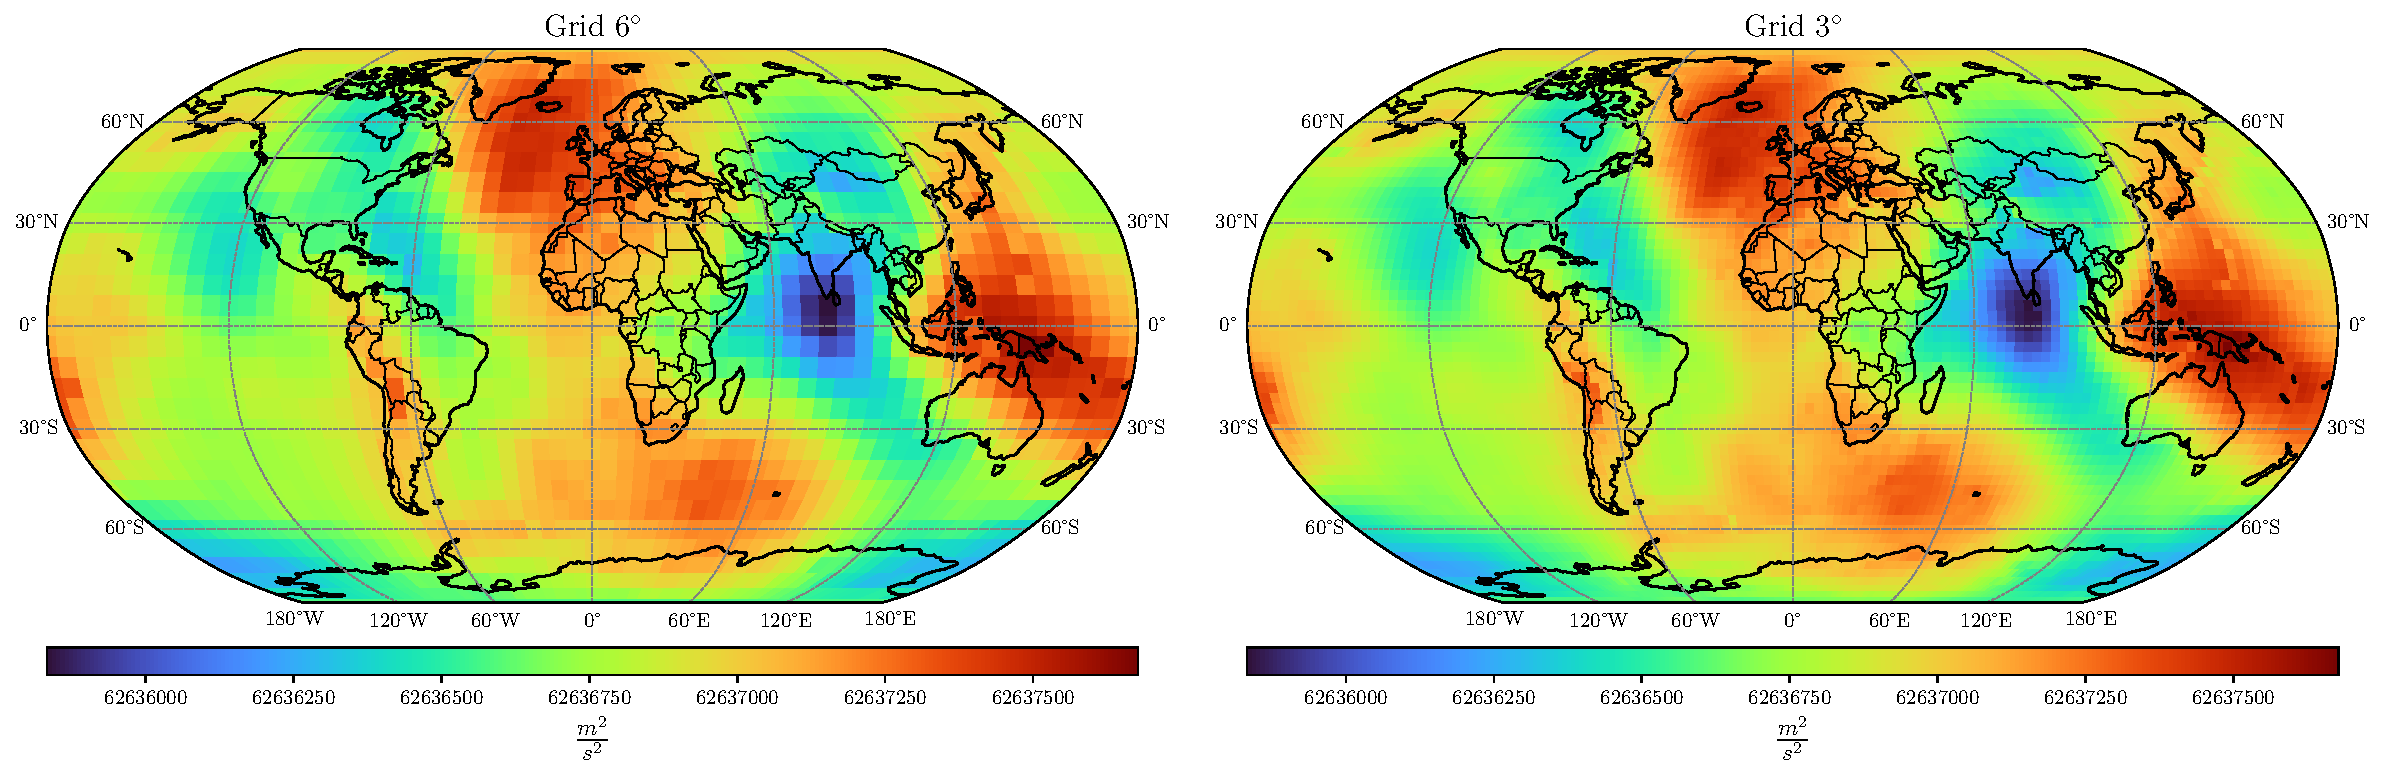
\includegraphics[width=16cm]{../Outputs/Plots/MainData.pdf}
		\caption{Gravity potential data used for interpolation and validation.}
		\label{fig:MainData}
	\end{figure}
	
	One of the main challenges of this project is determining the optimum value for parameter $h$. The method used here is a simple Cross-Validation (CV), where 5\% of input data was left aside from calculations and the norm of difference between interpolated value and true value for these points where taken into account for determining the best $h$, as shown in equation \ref{eq:CV}. In this equation, $S$ is the gravity potential values and $\hat{S}$ is the interpolated value for the validation points.
	
	\begin{equation}
		h_{opt} = \operatorname*{arg\,min}_{h} ||S-\hat{S}||_{2}
		\label{eq:CV}
	\end{equation}
	
	Different values for $h$ where tested in a manner of three steps. Firstly, values form $0.1$ to $0.9$ by step size of $0.1$ were tested. Then values around the result of previous step with the step size of 0.01 were tested. And Lastly the values by the step size of 0.001 around the result of the previous step were used. 
	
	The design matrix $A$ for solving coefficients is ill-conditioned, with the condition number in order of $10^{40}$ (Abel-Poisson kernel with $h=0.3$). The Picard plot for this matrix is shown in figure \ref{fig:PicardPlot}. 

	\begin{figure}[h!]
		\centering
		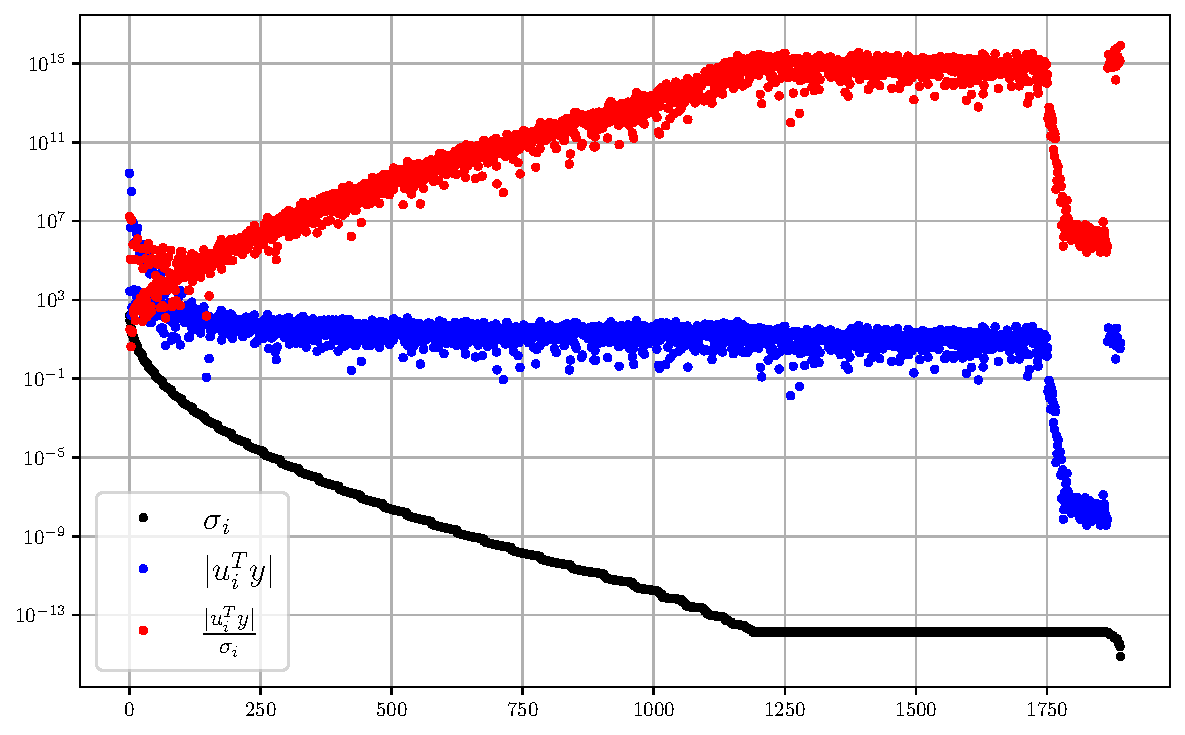
\includegraphics[height=3.8cm]{../Outputs/Plots/PicardPlot.pdf}
		\caption{Picard plot of the design matrix (Abel-Poisson kernel with $h=0.3$).}
		\label{fig:PicardPlot}
	\end{figure}
	
	Therefore methods of regularization is required for calculating the coefficients, and the solution by simply inverting the design matrix is not a reasonable solution, as shown in figure \ref{fig:NoRegResult}.  
	
	\begin{figure}[h!]
		\centering
		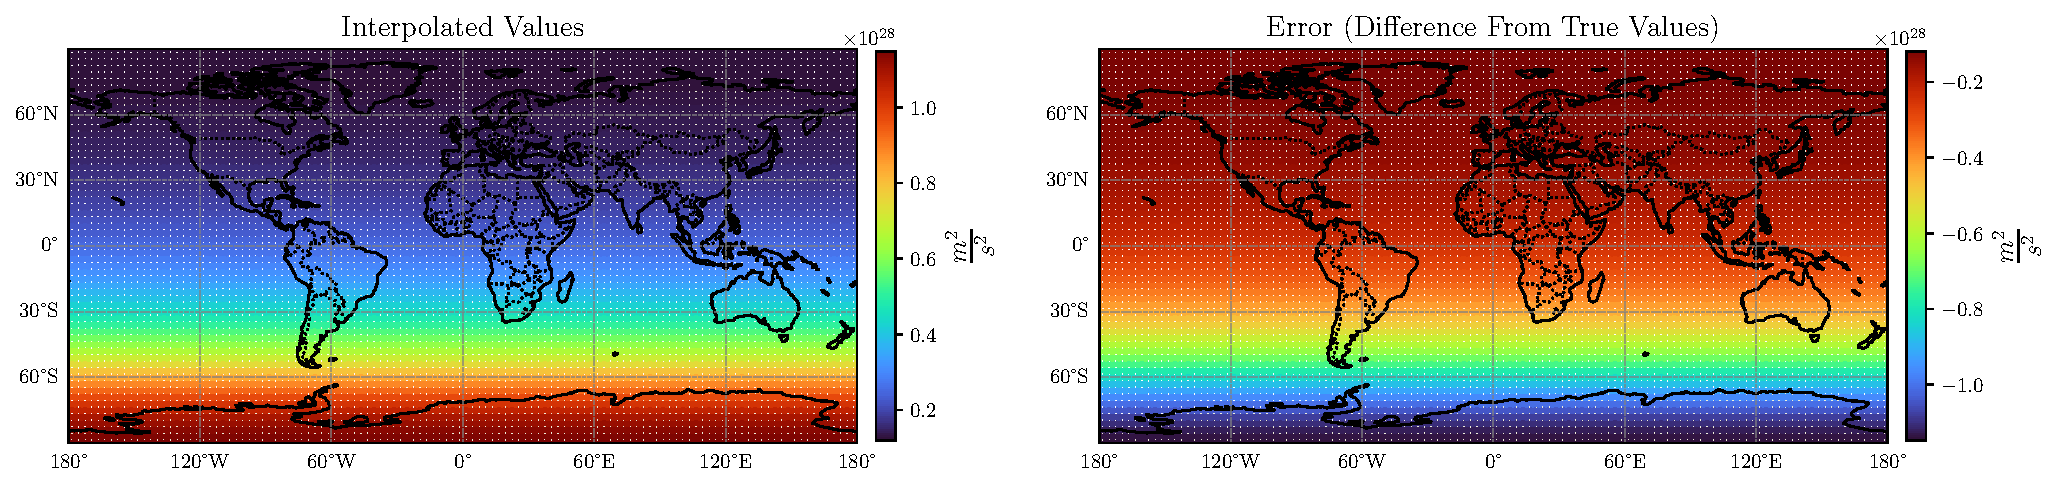
\includegraphics[height=5cm]{../Outputs/Plots/NoRegResult.pdf}
		\caption{Results without using regularization methods.}
		\label{fig:NoRegResult}
	\end{figure}
	
	Regularization methods used are TSVD and First order Tikhonov (FOT) With regularization parameter calculated from GCV, L-Curve and VCE methods. Cholesky decomposition is also used, which is a method for cases with numerical problems.
	

	
	Error of interpolation is defined as shown in equation \ref{eq:error}, Where $l$ is the true value acquired from XGM2019 model, and $\hat{l}$ is the interpolated value.
	
	\begin{equation}
		e = l - \hat{l}
		\label{eq:error}
	\end{equation}


	\section{Results}

	\subsection{Abel-Poisson}
	
	Interpolated and error values for Abel-Poisson kernel is shown in the figures \ref{fig:Abel-Poisson_Chol} to \ref{fig:Abel-Poisson_VCE}. The results for this kernel, including parameter $h$, regularization parameter, Mean and norm ($L^2$) of error are shown in table \ref{tab:Abel-Poisson_Results}. As it can be understood from the table, TSVD method was able to achieve the best result.
	
	\begin{table}[h!]
		\centering
		\caption{Results of interpolation using Abel-Poisson kernel (units of norm and mean values are $\frac{m^2}{s^2}$).}
		\vspace{0.2cm}
		\renewcommand{\arraystretch}{2}
		\begin{tabular}{c|c|c|c|c|c}
			\textbf{Method} & Cholesky & TSVD & GCV (FOT) & L-Curve (FOT) & VCE (FOT) \\
			\hline 
			\makecell{\textbf{Regularization} \\ \textbf{Parameter}} & --- & 1010 & $4.12*10^{-7}$ & $8.57*10^{-5}$ & $2.16*10^{-8}$ \\
			\hline 
			\textit{\textbf{h}} & 0.273 & 0.481 & 0.298 & 0.249 & 0.248 \\
			\hline
			\textbf{Mean of Error} & 0.2083 & \textcolor{blue}{0.1711} & -28.8998 & 2.5335 & 0.5352 \\
			\hline 
			\textbf{Norm of Errors} & 2076.6487 & \textcolor{blue}{2010.3925} & 4487.5036 & 7731.3095 & 5979.1538 \\
		\end{tabular}
		\label{tab:Abel-Poisson_Results}
	\end{table}
	
	\begin{figure}[h!]
		\centering
		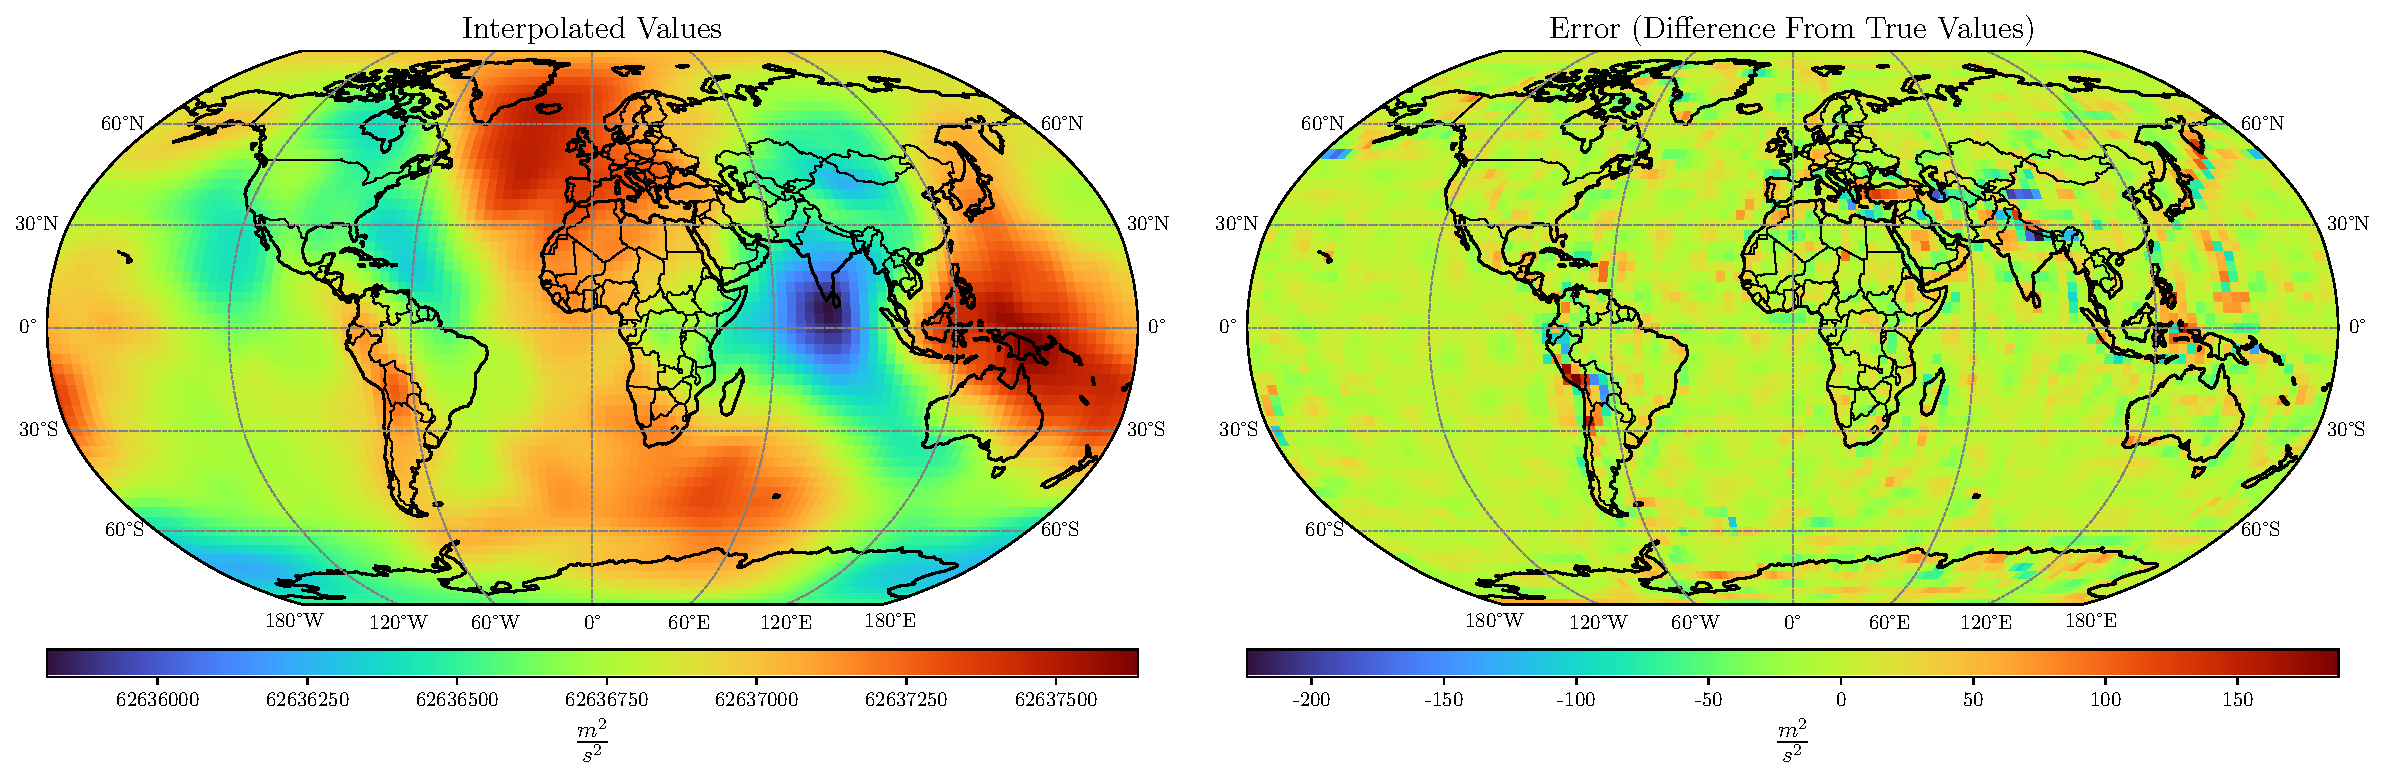
\includegraphics[width=16cm]{../Outputs/Plots/Plot_Abel-Poisson_Cholesky.pdf}
		\caption{Results of Abel-Poisson kernel with Cholesky decomposition.}
		\label{fig:Abel-Poisson_Chol}
	\end{figure}
	
	\begin{figure}[h!]
		\centering
		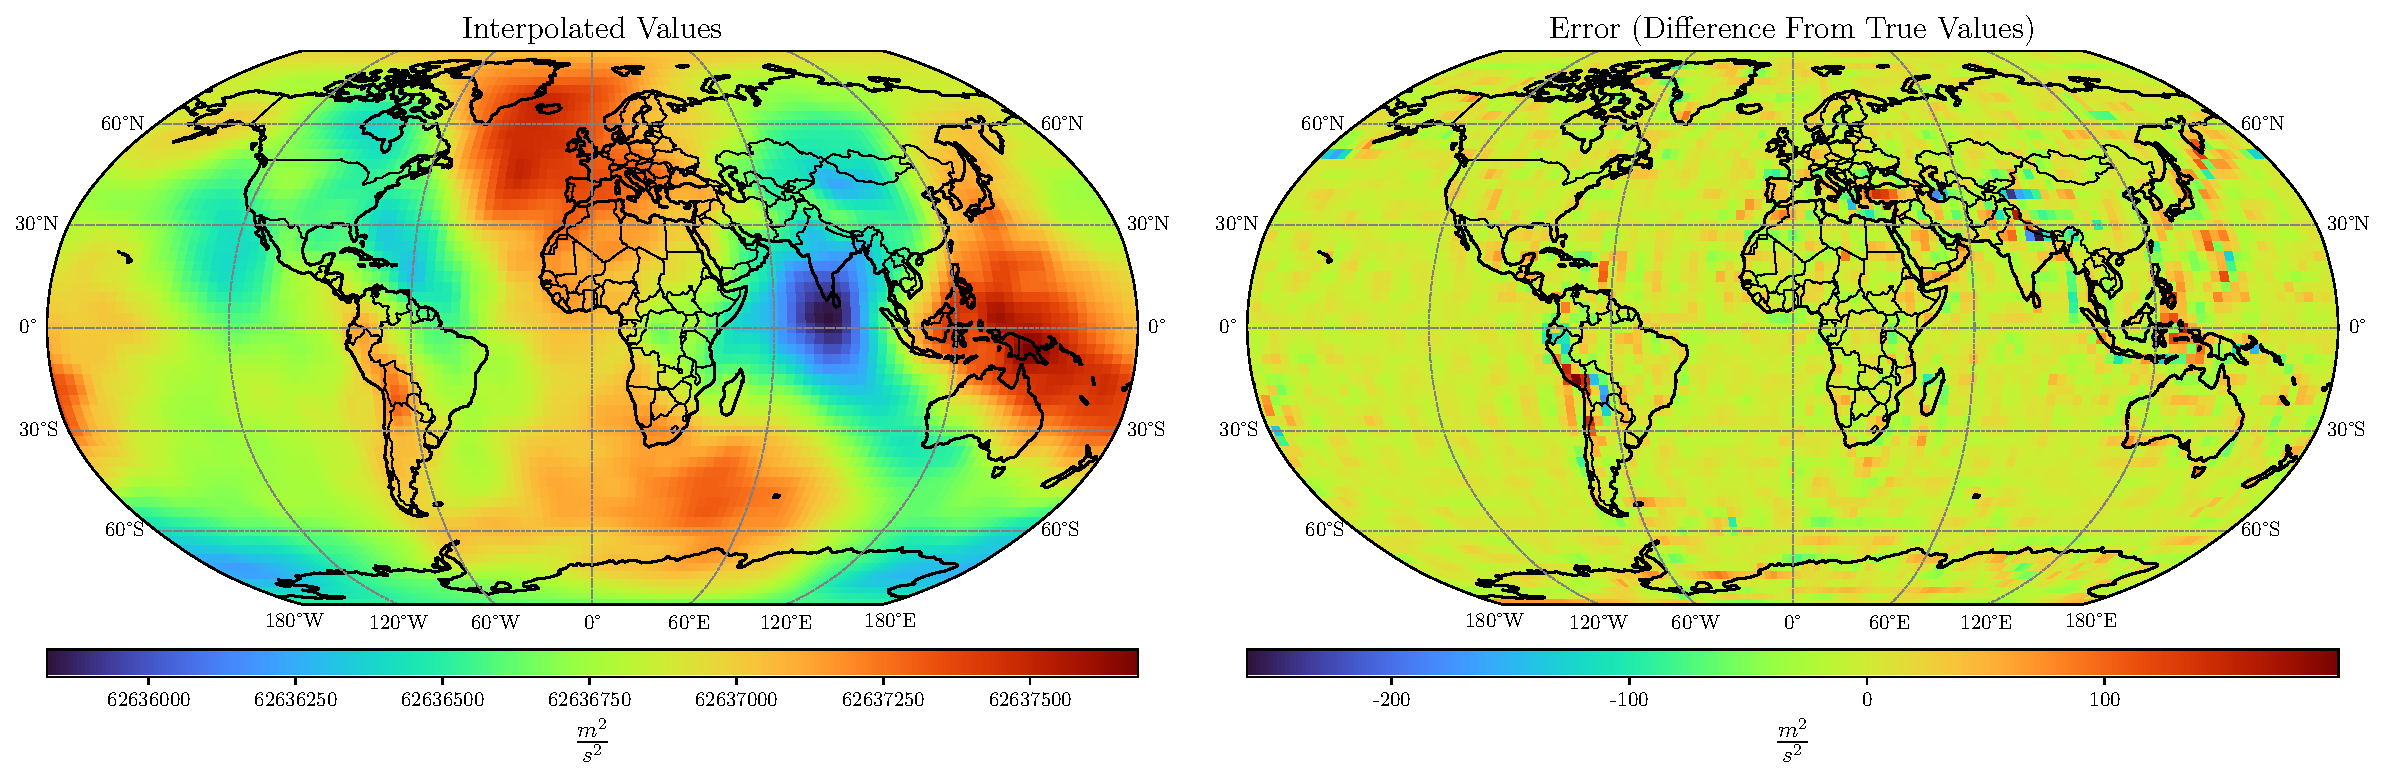
\includegraphics[width=16cm]{../Outputs/Plots/Plot_Abel-Poisson_TSVD.pdf}
		\caption{Results of Abel-Poisson kernel with TSVD method.}
		\label{fig:Abel-Poisson_TSVD}
	\end{figure}
	
	\clearpage
	
	\begin{figure}[h!]
		\centering
		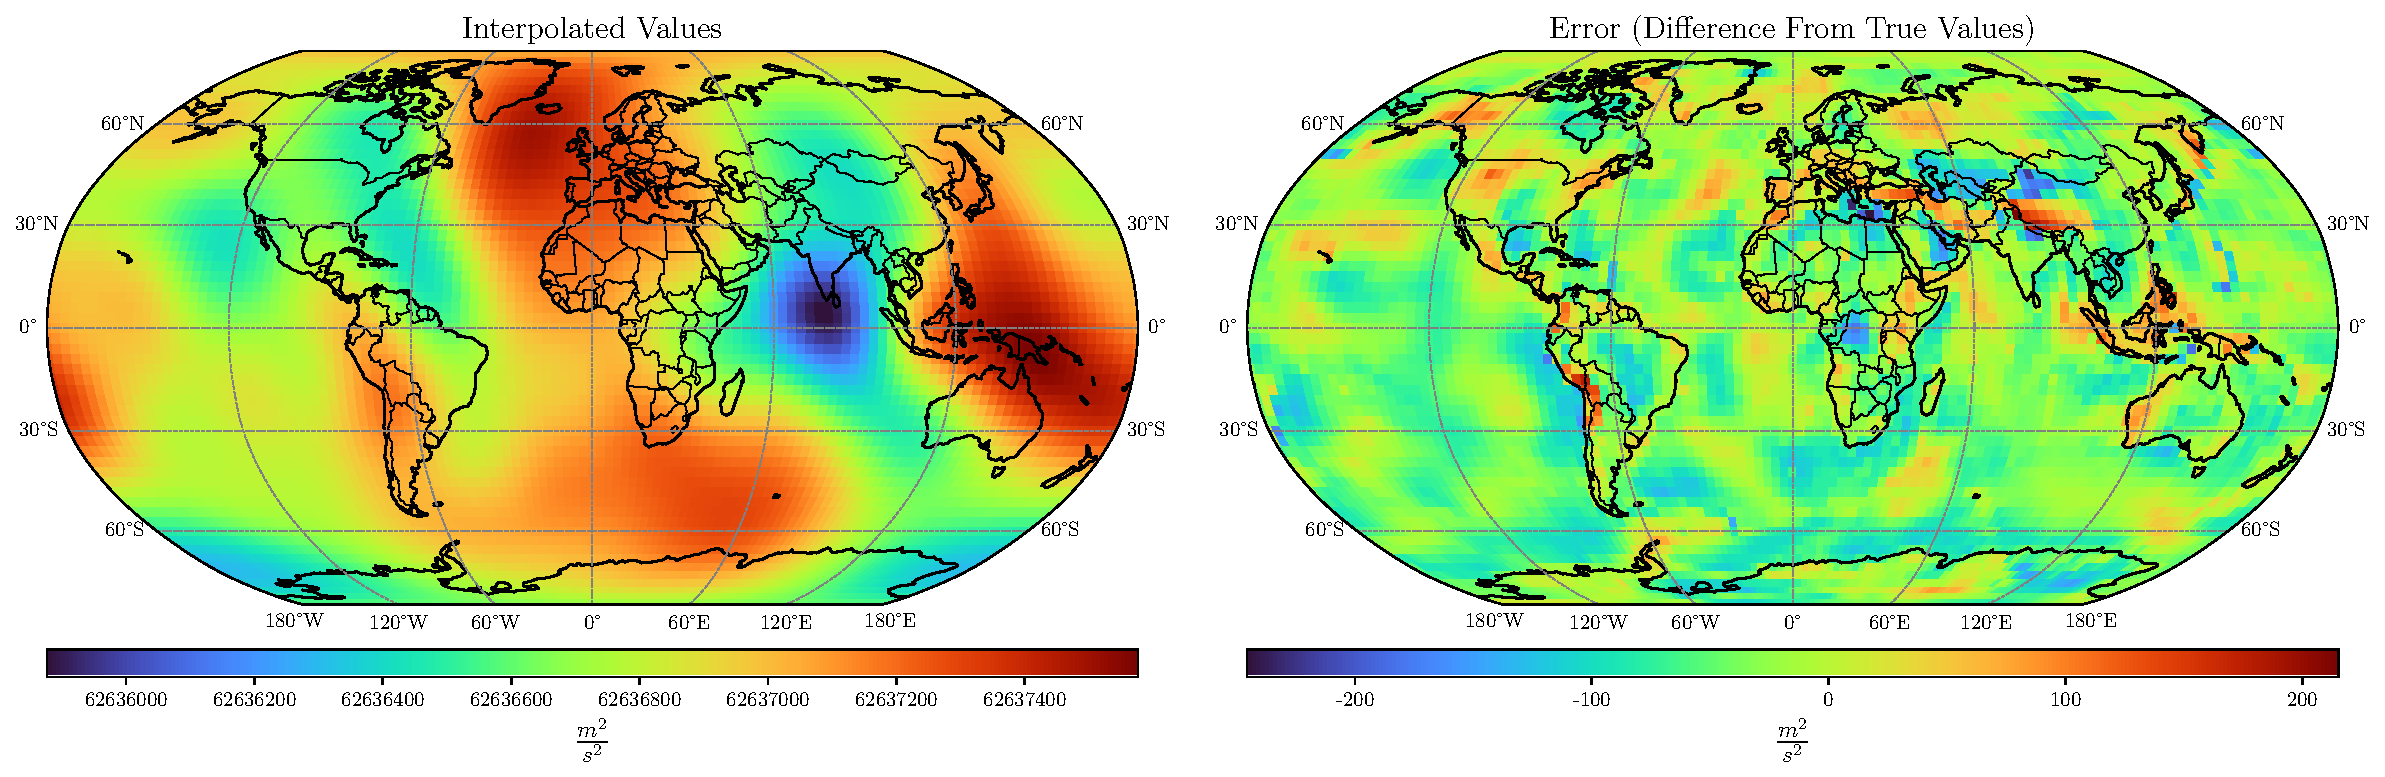
\includegraphics[width=16cm]{../Outputs/Plots/Plot_Abel-Poisson_GCV.pdf}
		\caption{Results of Abel-Poisson kernel with GCV (FOT) method.}
		\label{fig:Abel-Poisson_GCV}
	\end{figure}
	
	\begin{figure}[h!]
		\centering
		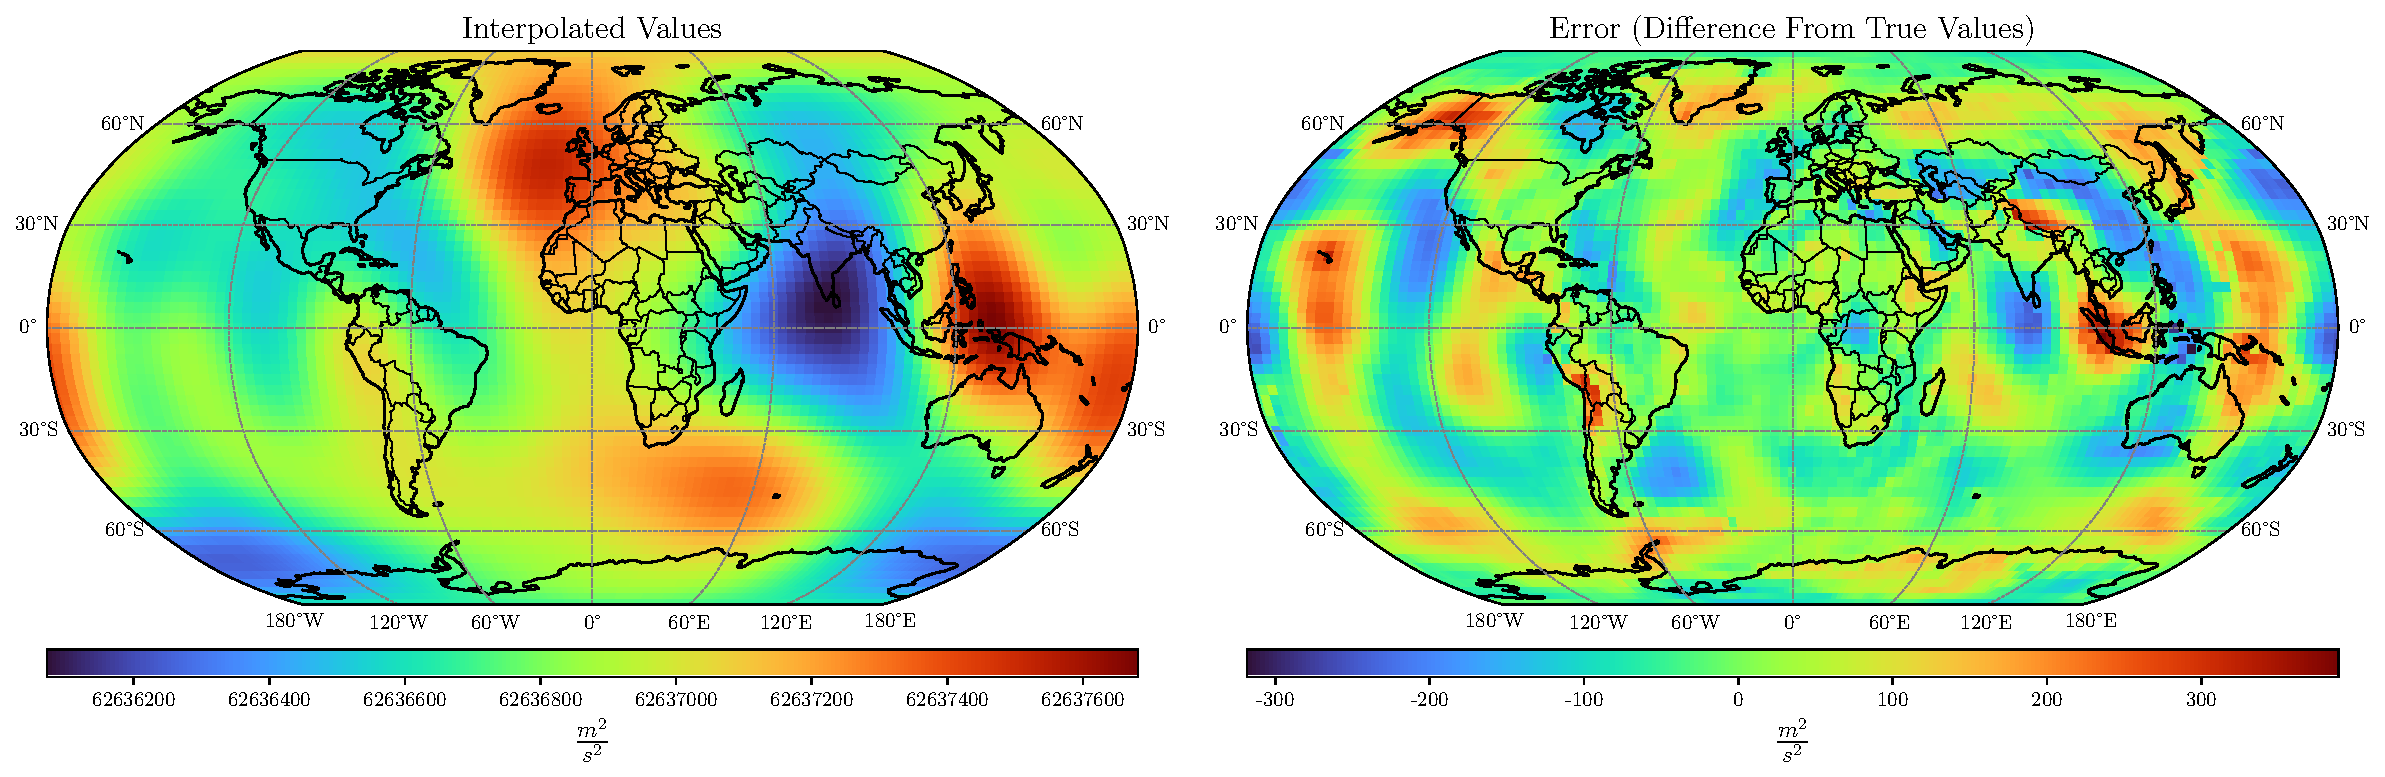
\includegraphics[width=16cm]{../Outputs/Plots/Plot_Abel-Poisson_L-Curve.pdf}
		\caption{Results of Abel-Poisson kernel with L-Curve (FOT) method.}
		\label{fig:Abel-Poisson_L-Curve}
	\end{figure}

	\begin{figure}[h!]
		\centering
		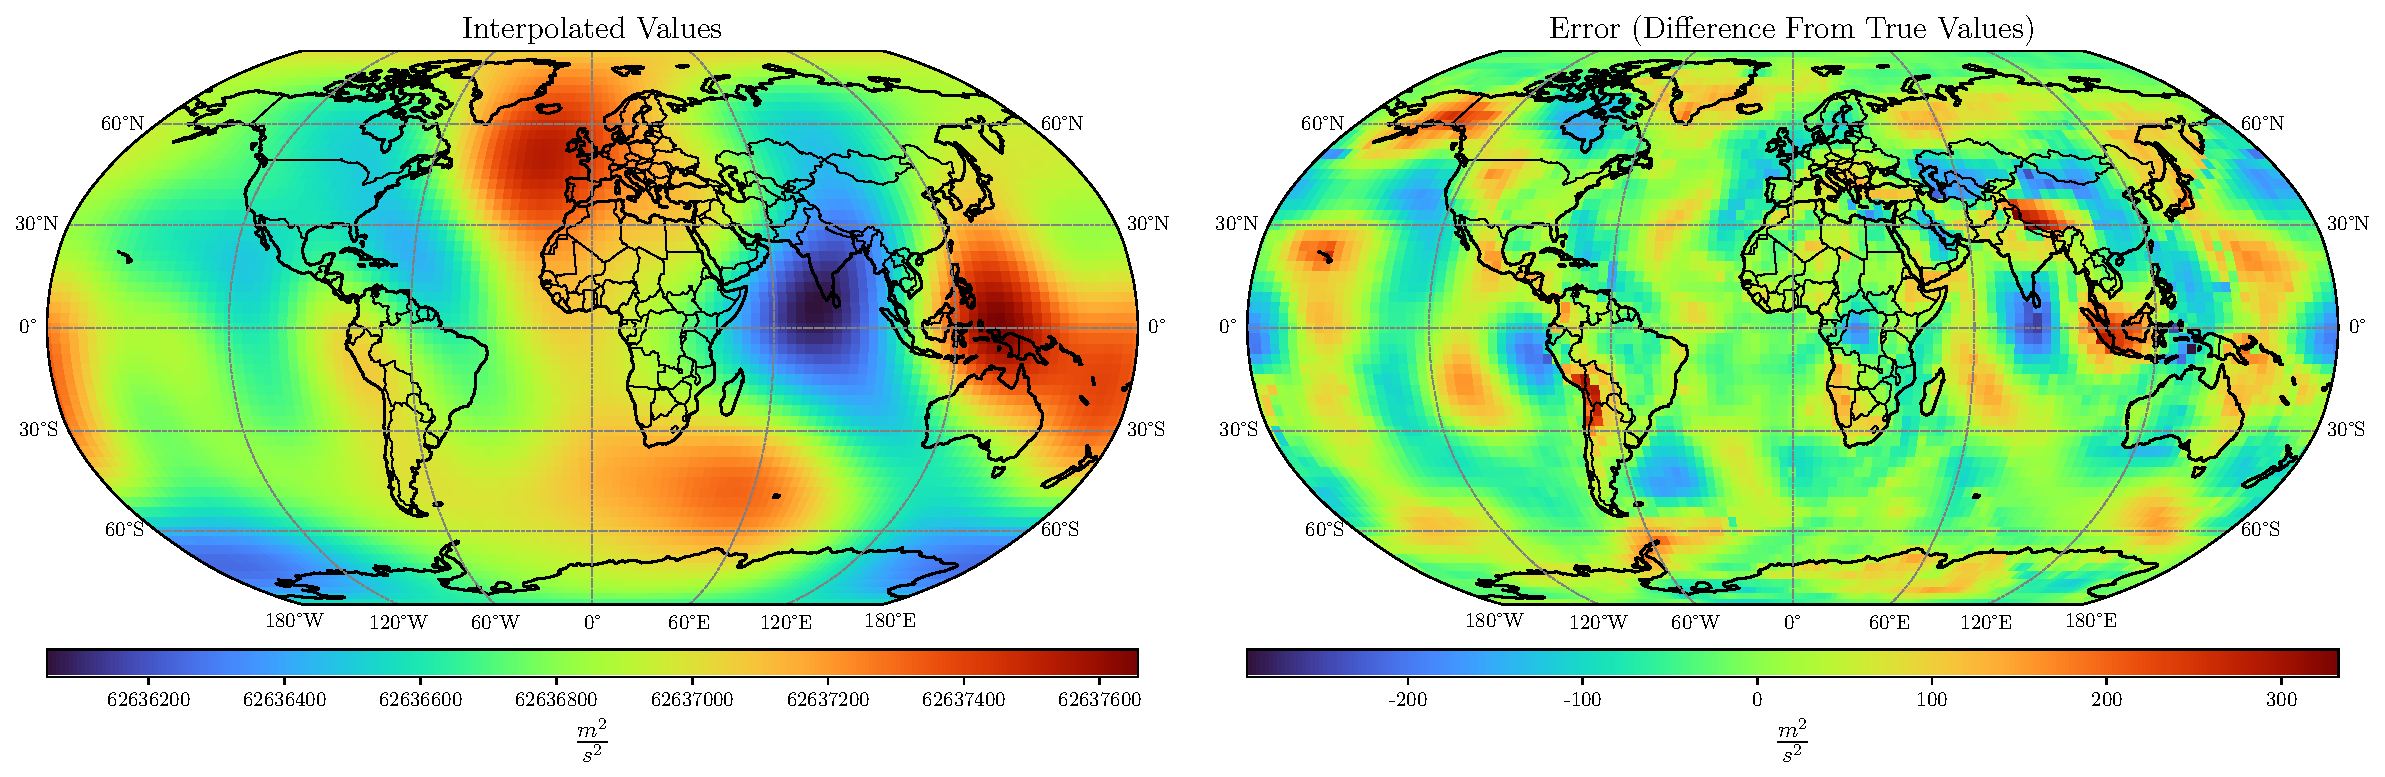
\includegraphics[width=16cm]{../Outputs/Plots/Plot_Abel-Poisson_VCE.pdf}
		\caption{Results of Abel-Poisson kernel with VCE (FOT) method.}
		\label{fig:Abel-Poisson_VCE}
	\end{figure}
	
	\subsection{Singularity}
	
	Interpolated and error values for Singularity kernel is shown in the figures \ref{fig:Singularity_Chol} to \ref{fig:Singularity_VCE}. The results for this kernel, including parameter $h$, regularization parameter, Mean and norm ($L^2$) of error are shown in table \ref{tab:Singularity_Results}. As it can be understood from the table, TSVD method was able to achieve the best result.
	
	\begin{table}[h!]
		\centering
		\caption{Results of interpolation using Singularity kernel (units of norm and mean values are $\frac{m^2}{s^2}$).}
		\vspace{0.2cm}
		\renewcommand{\arraystretch}{2}
		\begin{tabular}{c|c|c|c|c|c}
			\textbf{Method} & Cholesky & TSVD & GCV (FOT) & L-Curve (FOT) & VCE (FOT) \\
			\hline 
			\makecell{\textbf{Regularization} \\ \textbf{Parameter}} & --- & 1005 & $4.26*10^{-6}$ & $1.43*10^{-4}$ & $3.27*10^{-8}$ \\
			\hline 
			\textit{\textbf{h}} & 0.264 & 0.429 & 0.364 & 0.427 & 0.440 \\
			\hline
			\textbf{Mean of Error} & 0.2437 & \textcolor{blue}{0.1703} & 9.1348 & 1.8637 & 5.5732 \\
			\hline 
			\textbf{Norm of Errors} & 2167.4400 & \textcolor{blue}{2013.2368} & 4211.3836 & 5557.0321 & 3745.0423 \\
		\end{tabular}
		\label{tab:Singularity_Results}
	\end{table}
	
	
	\begin{figure}[h!]
		\centering
		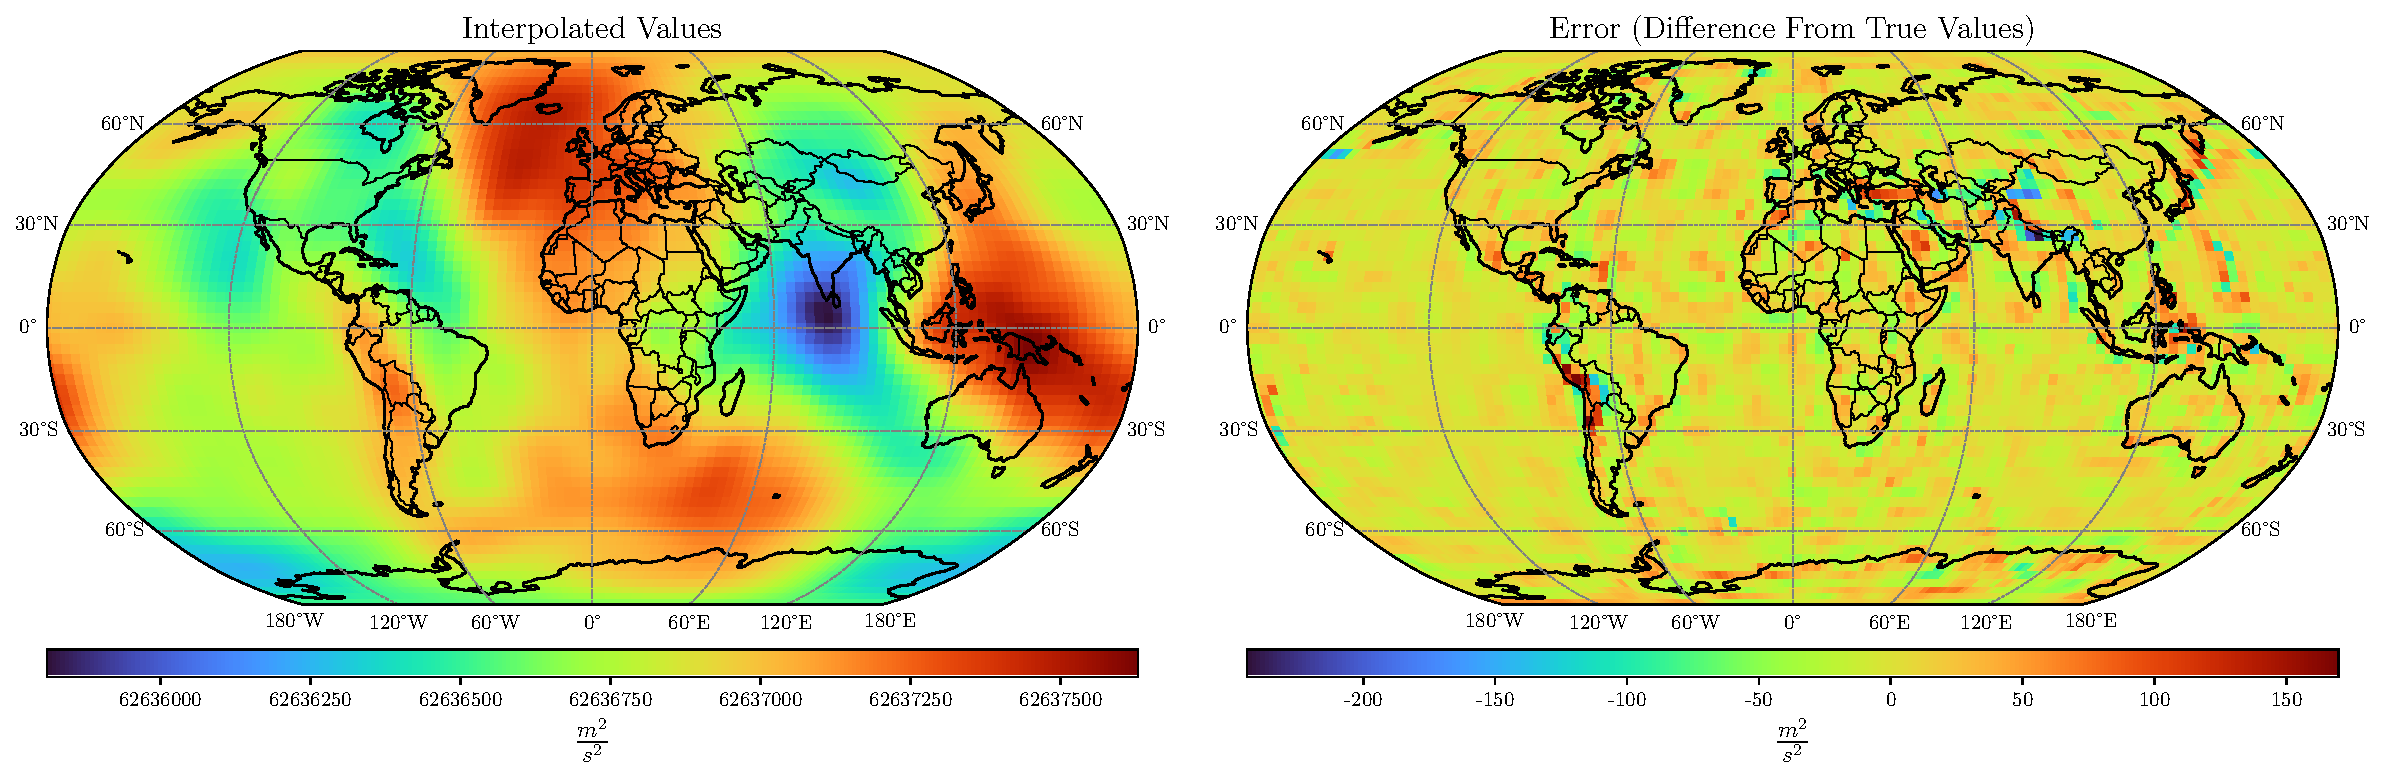
\includegraphics[width=16cm]{../Outputs/Plots/Plot_Singularity_Cholesky.pdf}
		\caption{Results of Singularity kernel with Cholesky decomposition.}
		\label{fig:Singularity_Chol}
	\end{figure}
	
	\begin{figure}[h!]
		\centering
		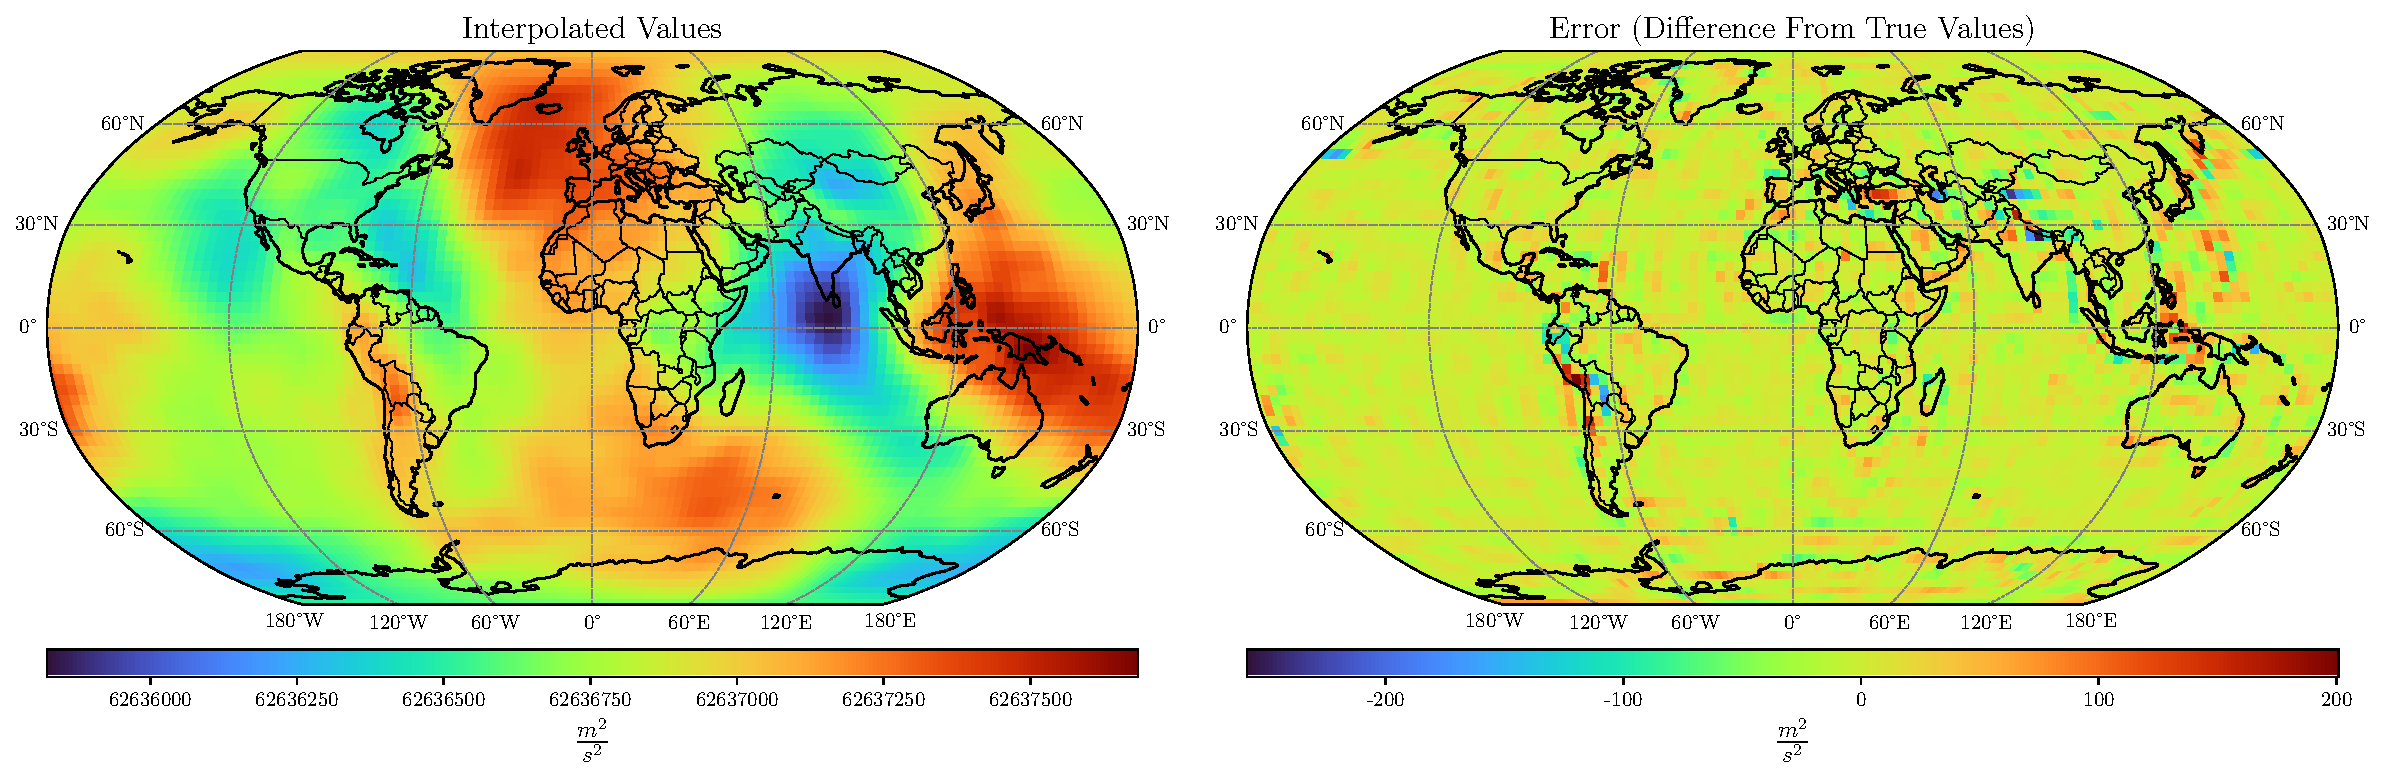
\includegraphics[width=16cm]{../Outputs/Plots/Plot_Singularity_TSVD.pdf}
		\caption{Results of Singularity kernel with TSVD method.}
		\label{fig:Singularity_TSVD}
	\end{figure}
	
	\clearpage
	
	\begin{figure}[h!]
		\centering
		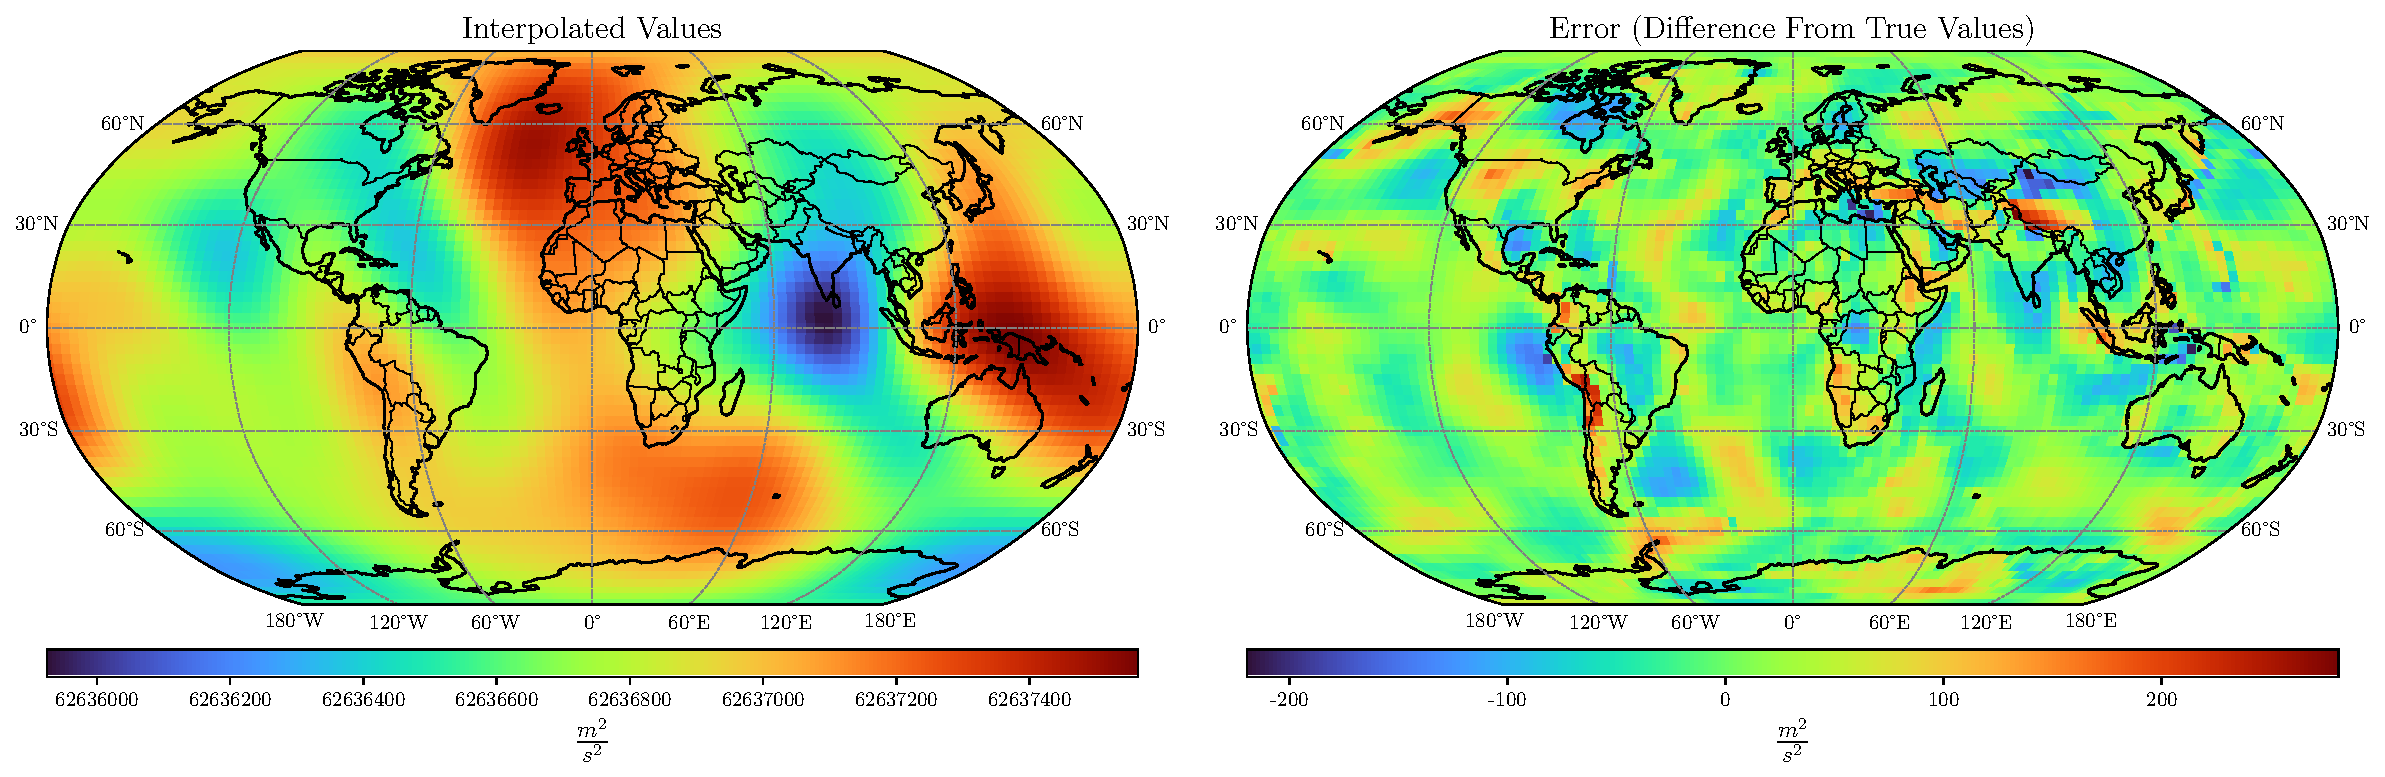
\includegraphics[width=16cm]{../Outputs/Plots/Plot_Singularity_GCV.pdf}
		\caption{Results of Singularity kernel with GCV (FOT) method.}
		\label{fig:Singularity_GCV}
	\end{figure}
	
	\begin{figure}[h!]
		\centering
		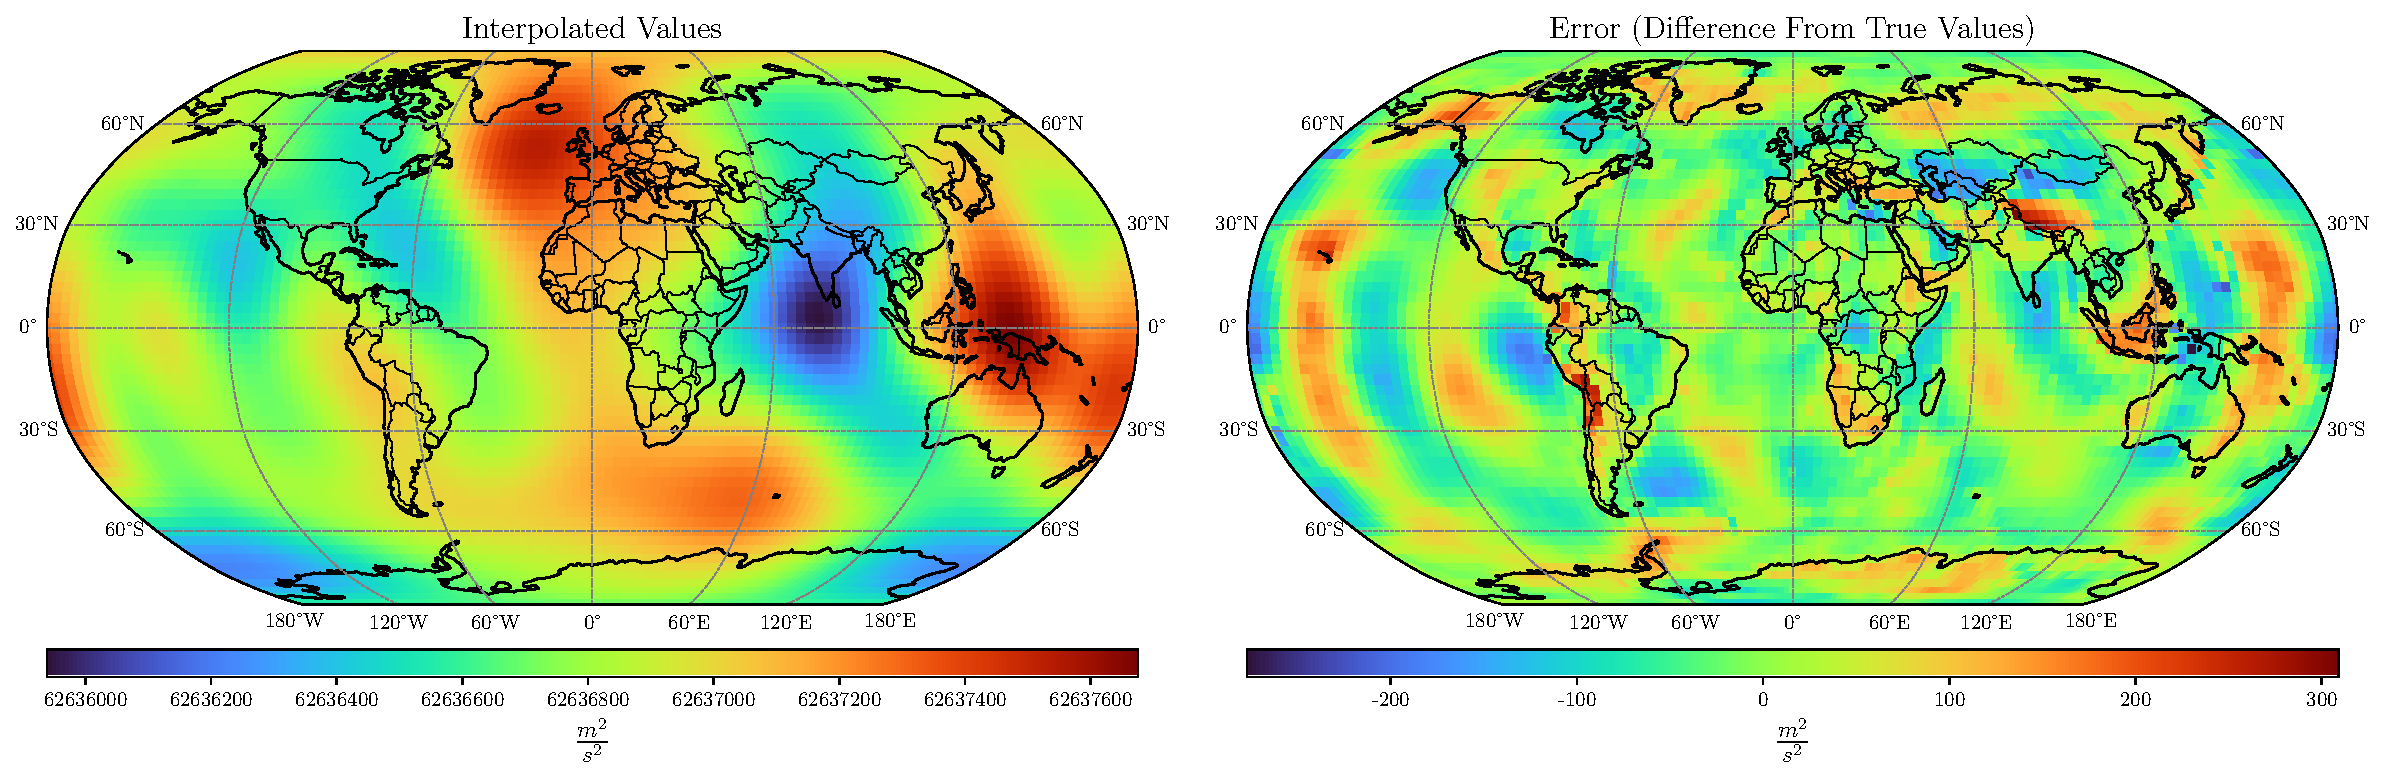
\includegraphics[width=16cm]{../Outputs/Plots/Plot_Singularity_L-Curve.pdf}
		\caption{Results of Singularity kernel with L-Curve (FOT) method.}
		\label{fig:Singularity_L-Curve}
	\end{figure}
	
	\begin{figure}[h!]
		\centering
		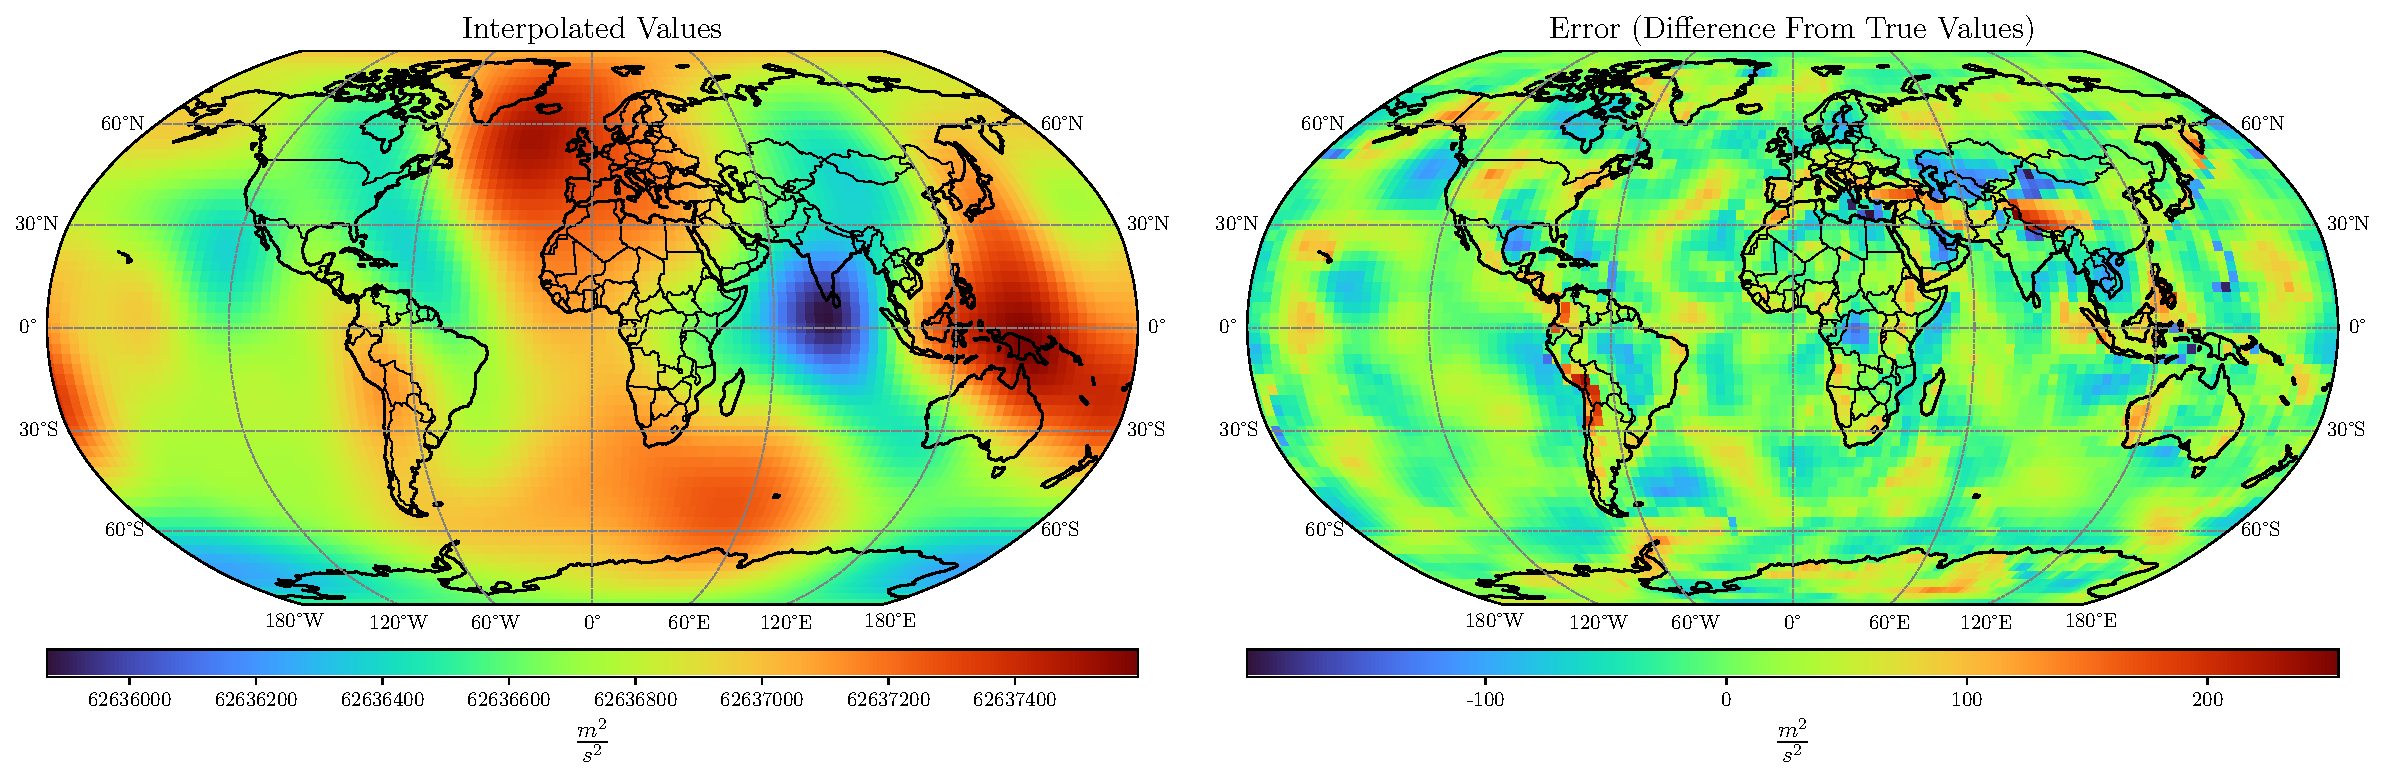
\includegraphics[width=16cm]{../Outputs/Plots/Plot_Singularity_VCE.pdf}
		\caption{Results of Singularity kernel with VCE (FOT) method.}
		\label{fig:Singularity_VCE}
	\end{figure}
	
	\subsection{Logarithmic}
	
	Interpolated and error values for Logarithmic kernel is shown in the figures \ref{fig:Logarithmic_Chol} to \ref{fig:Logarithmic_VCE}. The results for this kernel, including parameter $h$, regularization parameter, Mean and norm ($L^2$) of error are shown in table \ref{tab:Logarithmic_Results}. As it can be understood from the table, TSVD method was able to achieve the best result.
	
	\begin{table}[h!]
		\centering
		\caption{Results of interpolation using Logarithmic kernel (units of norm and mean values are $\frac{m^2}{s^2}$).}
		\vspace{0.2cm}
		\renewcommand{\arraystretch}{2}
		\begin{tabular}{c|c|c|c|c|c}
			\textbf{Method} & Cholesky & TSVD & GCV (FOT) & L-Curve (FOT) & VCE (FOT) \\
			\hline 
			\makecell{\textbf{Regularization} \\ \textbf{Parameter}} & --- & 1010 & $7.96*10^{-7}$ & $1.20*10^{-4}$ & $1.47*10^{-7}$ \\
			\hline 
			\textit{\textbf{h}} & 0.286 & 0.559 & 0.411 & 0.535 & 0.367 \\
			\hline
			\textbf{Mean of Error} & 0.2559 & \textcolor{blue}{0.1712} & 57.395 & 1.8417 & 1.3222 \\
			\hline 
			\textbf{Norm of Errors} & 2220.5339 & \textcolor{blue}{2007.4311} & 6614.5388 & 5723.9421 & 7804.3402 \\
		\end{tabular}
		\label{tab:Logarithmic_Results}
	\end{table}
	
	\begin{figure}[h!]
		\centering
		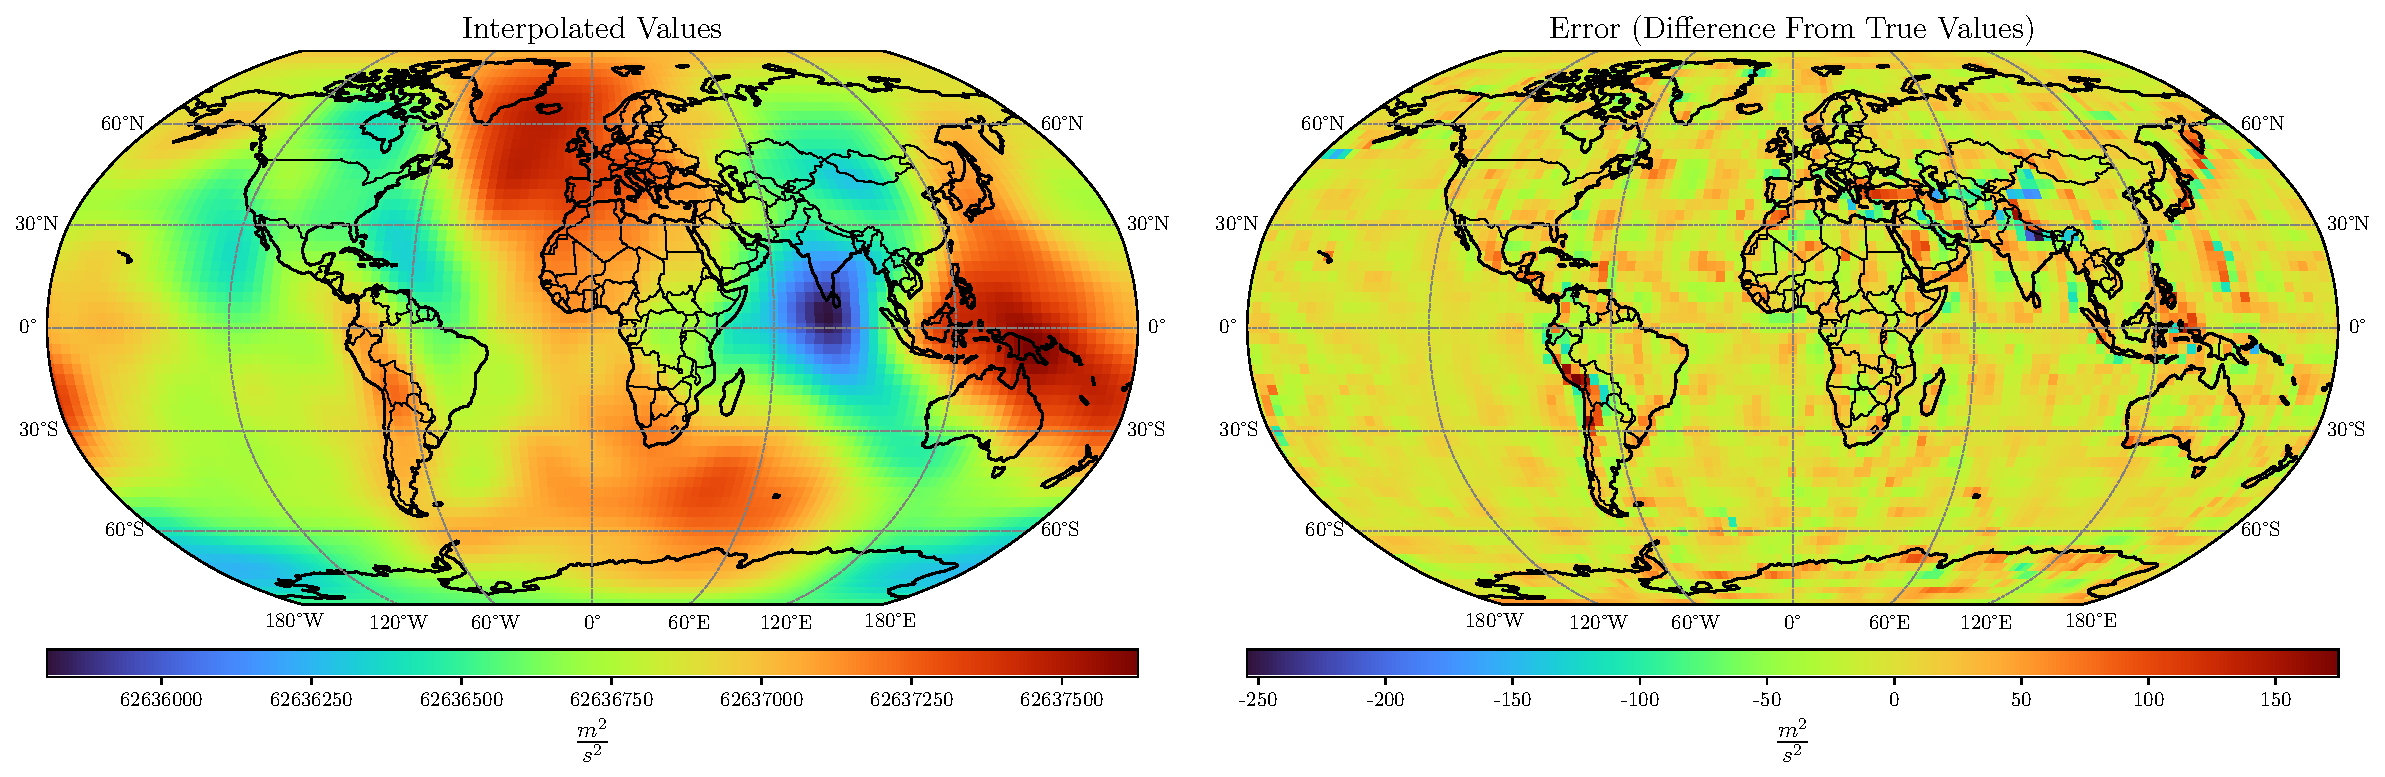
\includegraphics[width=16cm]{../Outputs/Plots/Plot_Logarithmic_Cholesky.pdf}
		\caption{Results of Logarithmic kernel with Cholesky decomposition.}
		\label{fig:Logarithmic_Chol}
	\end{figure}
	
	\begin{figure}[h!]
		\centering
		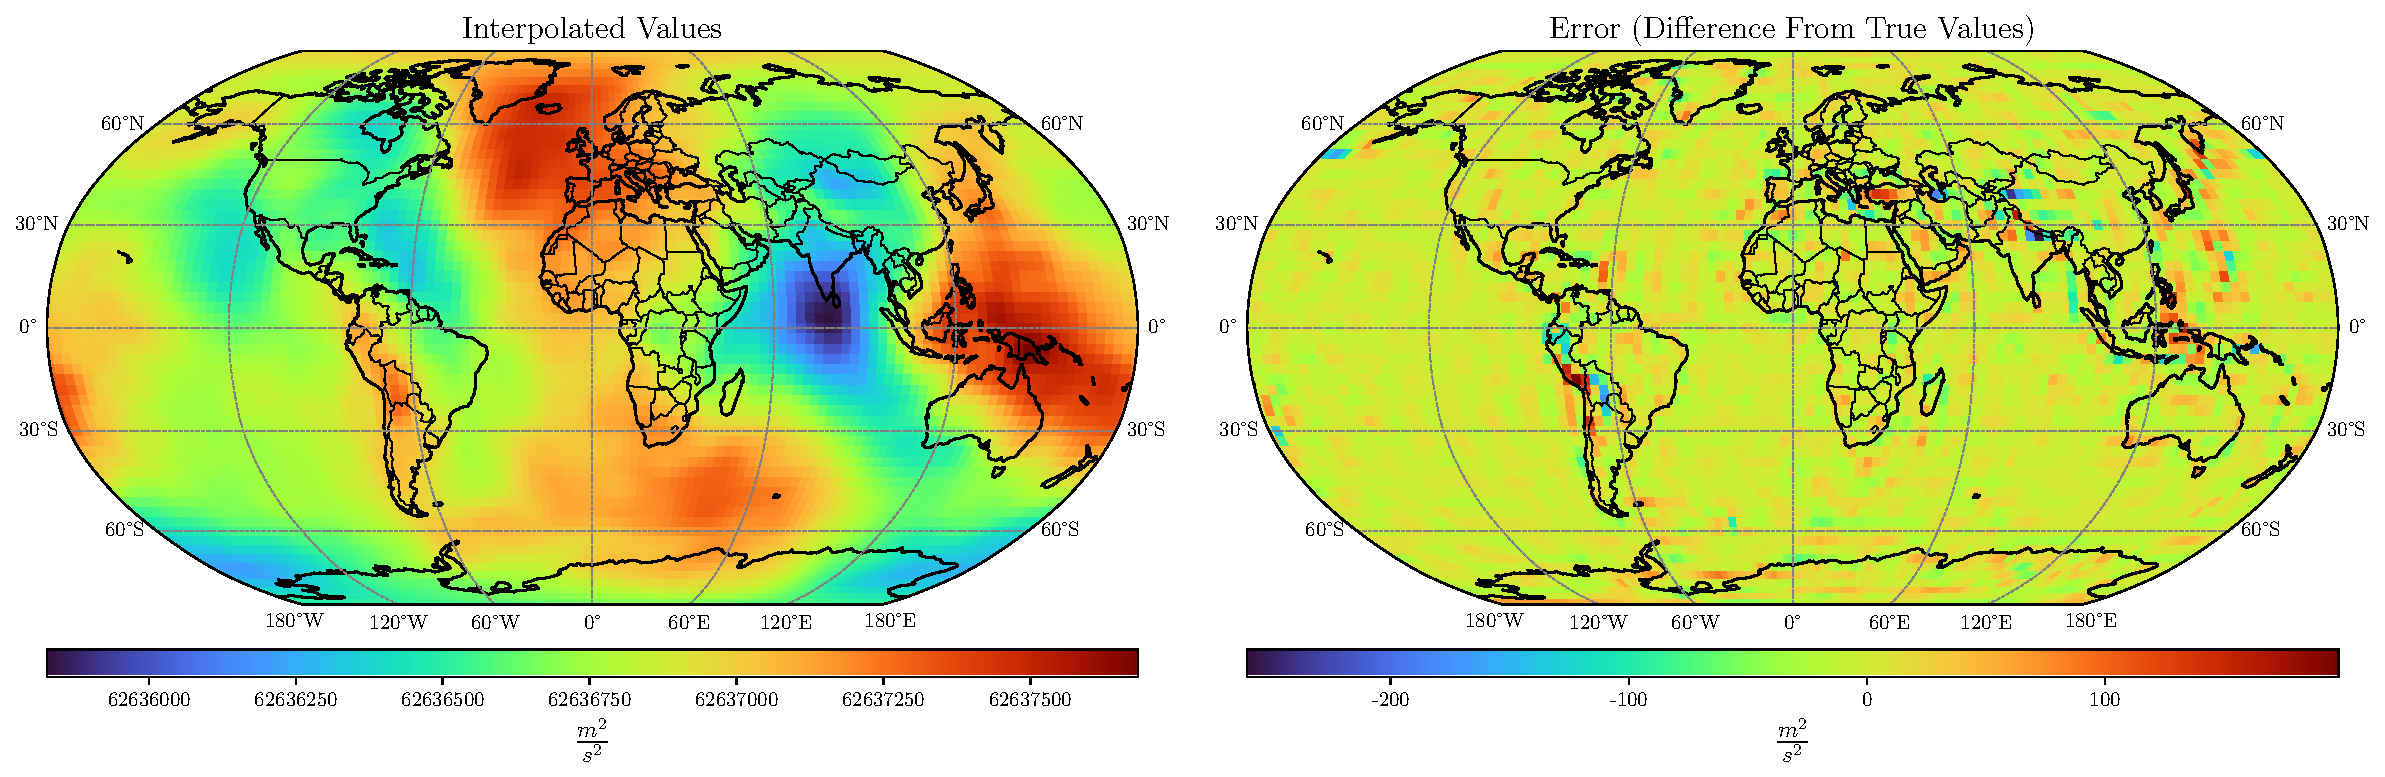
\includegraphics[width=16cm]{../Outputs/Plots/Plot_Logarithmic_TSVD.pdf}
		\caption{Results of Logarithmic kernel with TSVD method.}
		\label{fig:Logarithmic_TSVD}
	\end{figure}
	
	\clearpage
	
	\begin{figure}[h!]
		\centering
		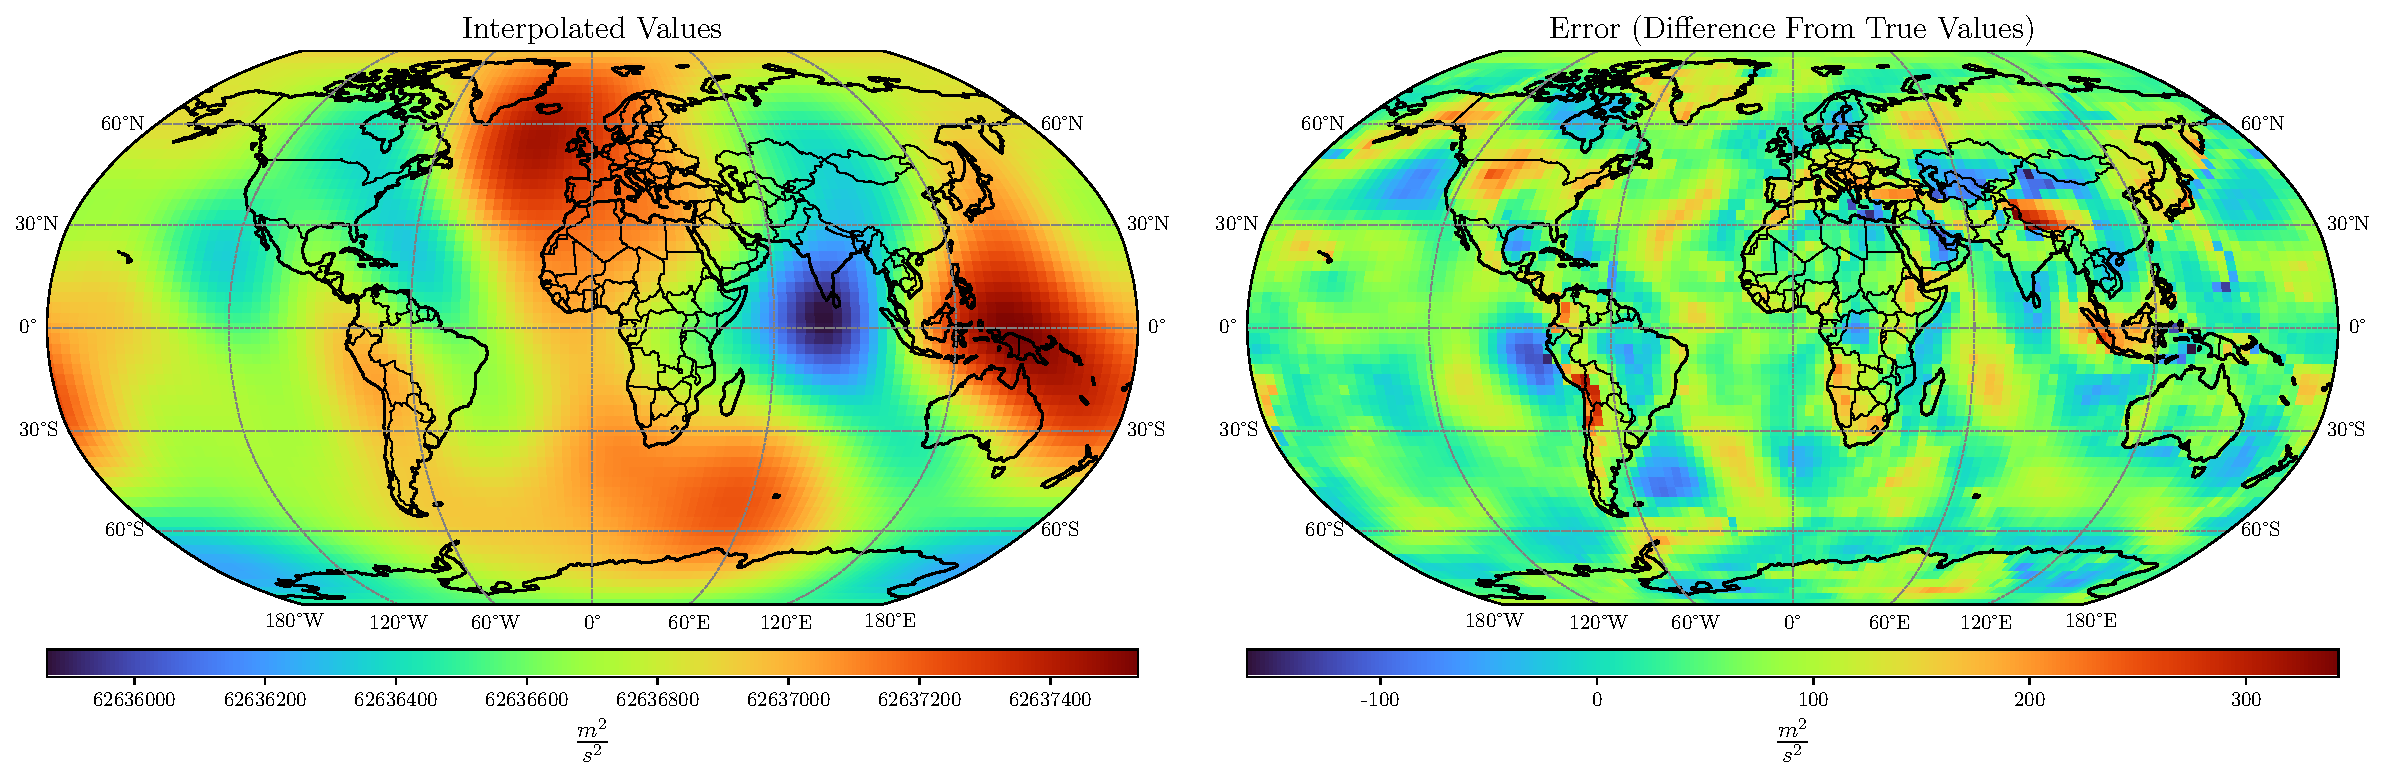
\includegraphics[width=16cm]{../Outputs/Plots/Plot_Logarithmic_GCV.pdf}
		\caption{Results of Logarithmic kernel with GCV (FOT) method.}
		\label{fig:Logarithmic_GCV}
	\end{figure}
	
	\begin{figure}[h!]
		\centering
		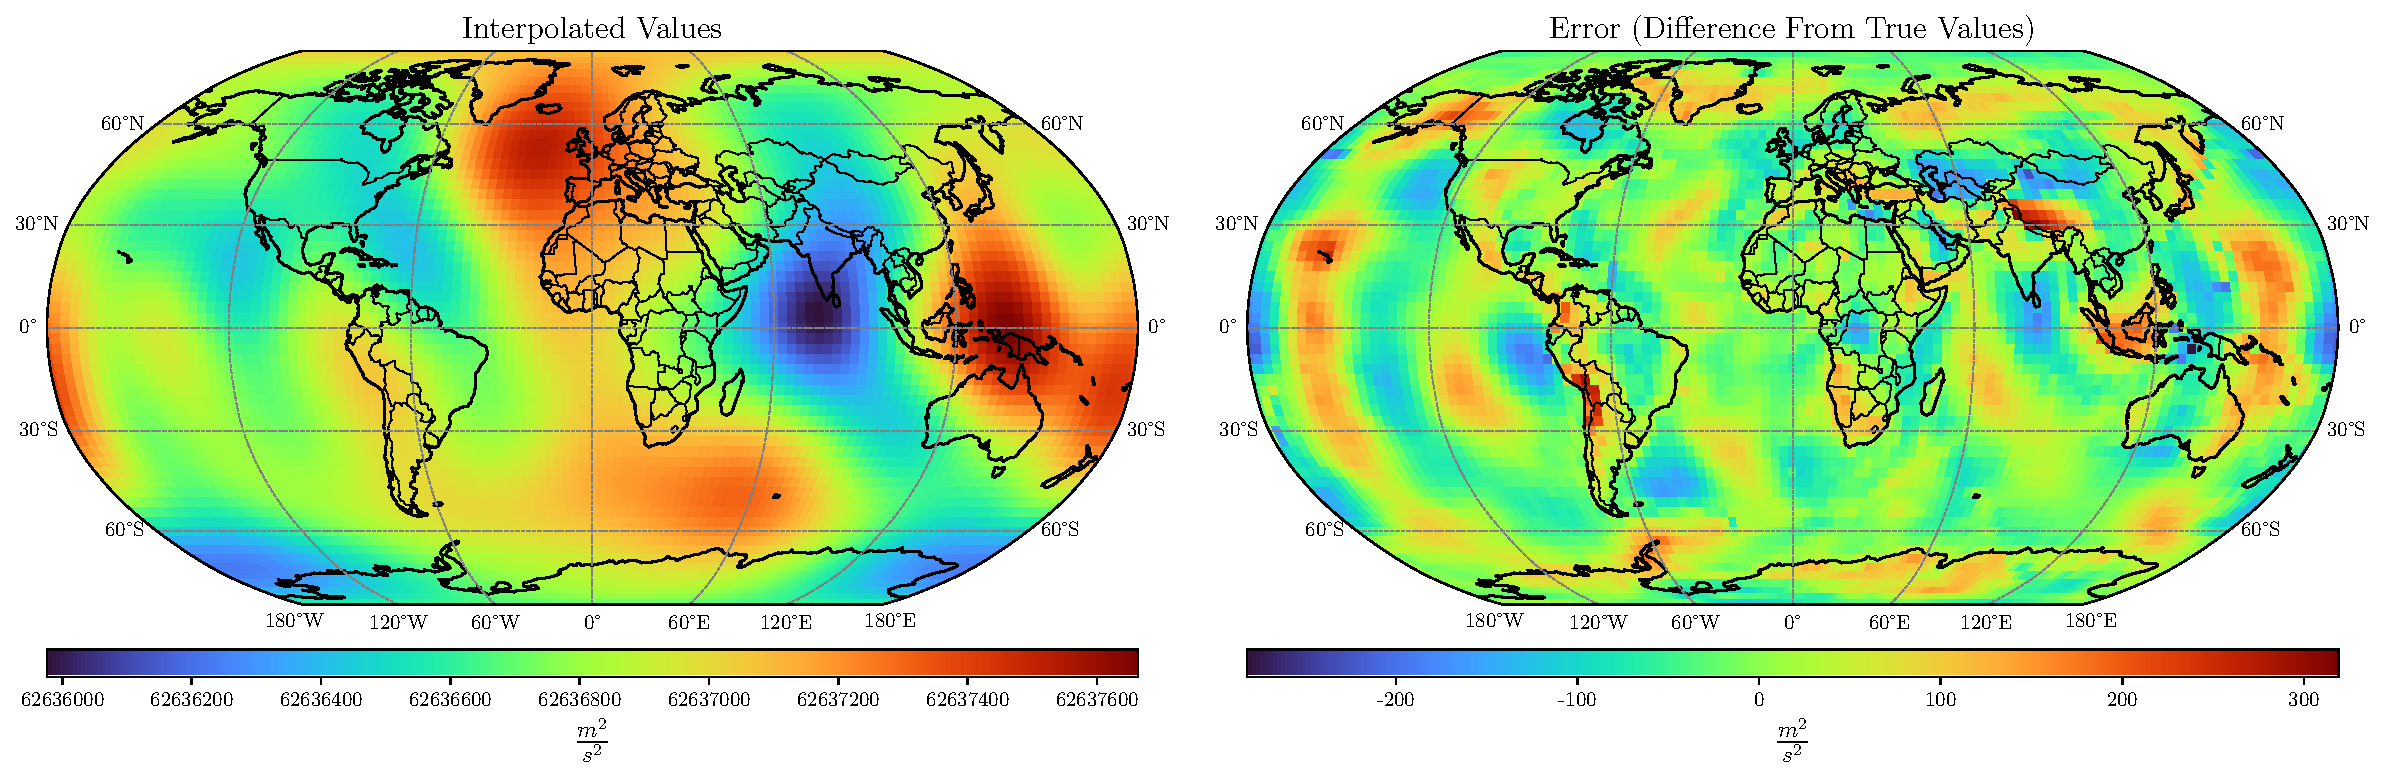
\includegraphics[width=16cm]{../Outputs/Plots/Plot_Logarithmic_L-Curve.pdf}
		\caption{Results of Logarithmic kernel with L-Curve (FOT) method.}
		\label{fig:Logarithmic_L-Curve}
	\end{figure}
	
	\begin{figure}[h!]
		\centering
		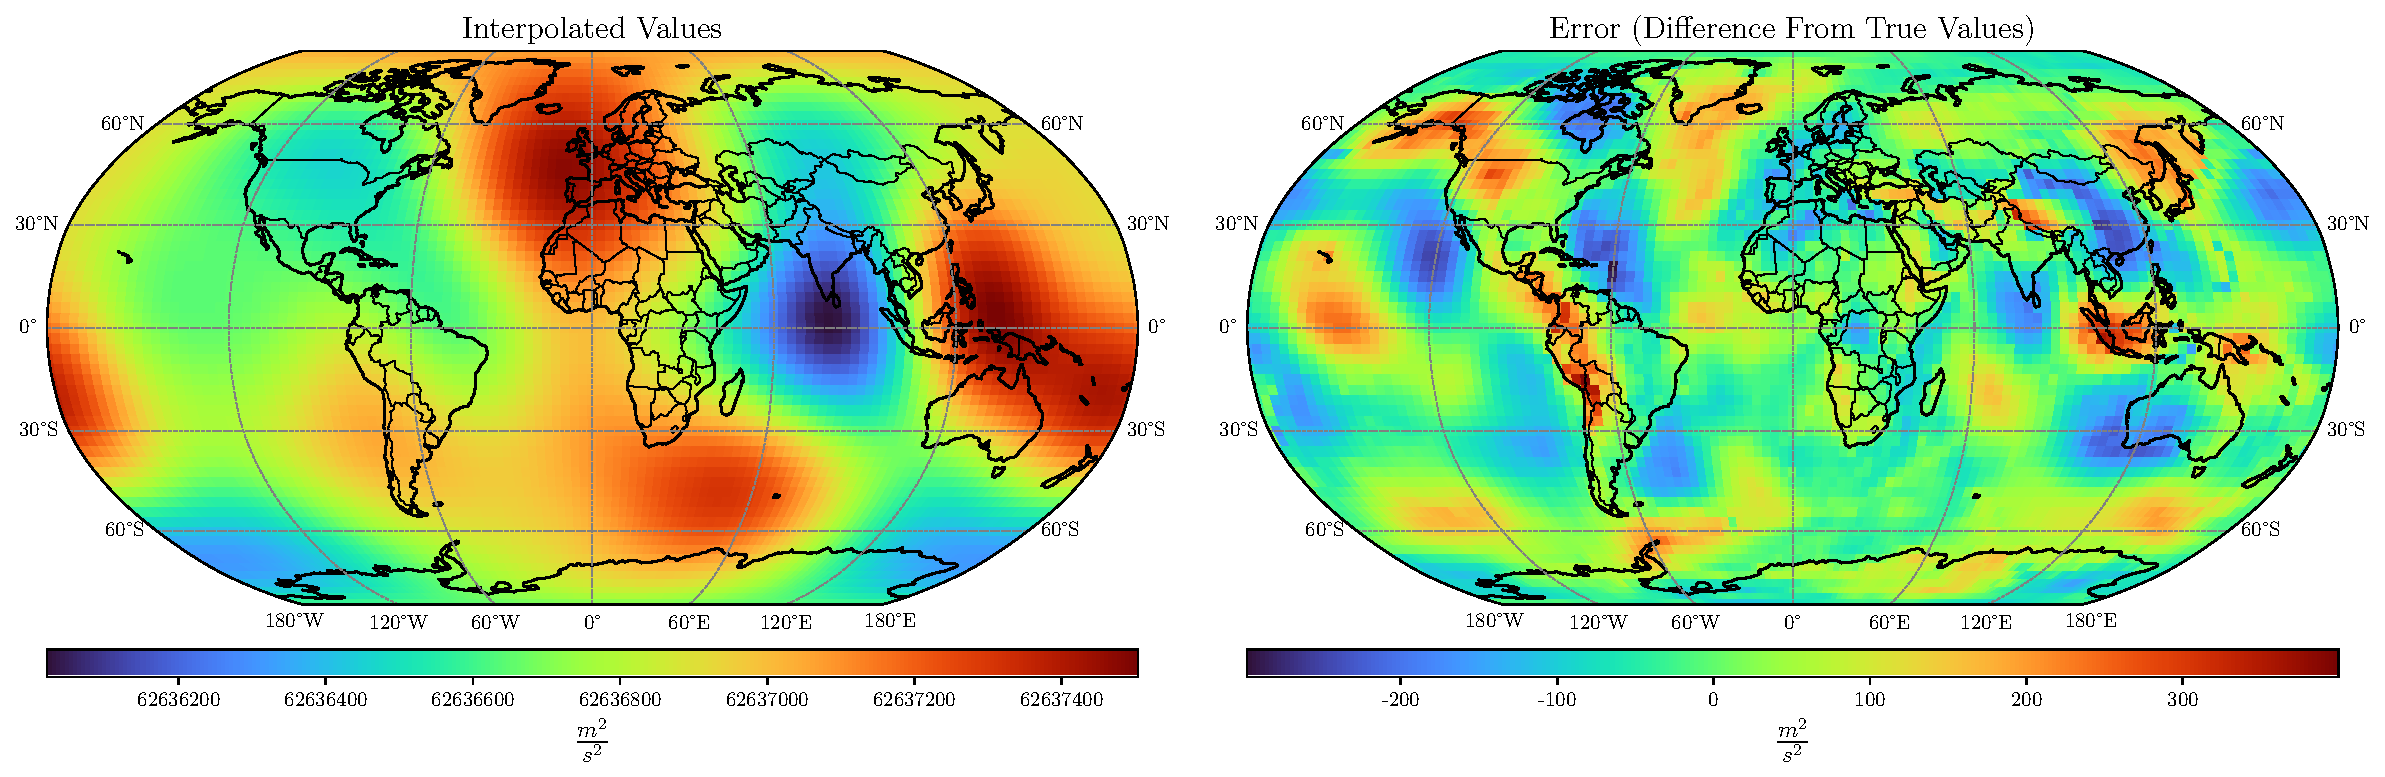
\includegraphics[width=16cm]{../Outputs/Plots/Plot_Logarithmic_VCE.pdf}
		\caption{Results of Logarithmic kernel with VCE (FOT) method.}
		\label{fig:Logarithmic_VCE}
	\end{figure}
	
	\subsection{Abel-Poisson With Noise}
	
	In this case, white-noise with standard deviation of $200 \frac{m^2}{s^2}$ was added to the input values, the noisy input data is shown in figure \ref{fig:DataWithNoise}. Interpolated and error values are shown in the figures \ref{fig:wn_Abel-Poisson_Chol} to \ref{fig:wn_Abel-Poisson_VCE}. Other results, including parameter $h$, regularization parameter, Mean and norm ($L^2$) of error are shown in table \ref{tab:wn_Abel-Poisson_Results}. As it can be understood from the table, TSVD and Cholesky methods were able to achieve the best results. Furthermore, results from other methods are too smooth and not reliable. 
	Between FOT methods, VCE could result in better answer than other two methods.
	
	\begin{figure}[h!]
		\centering
		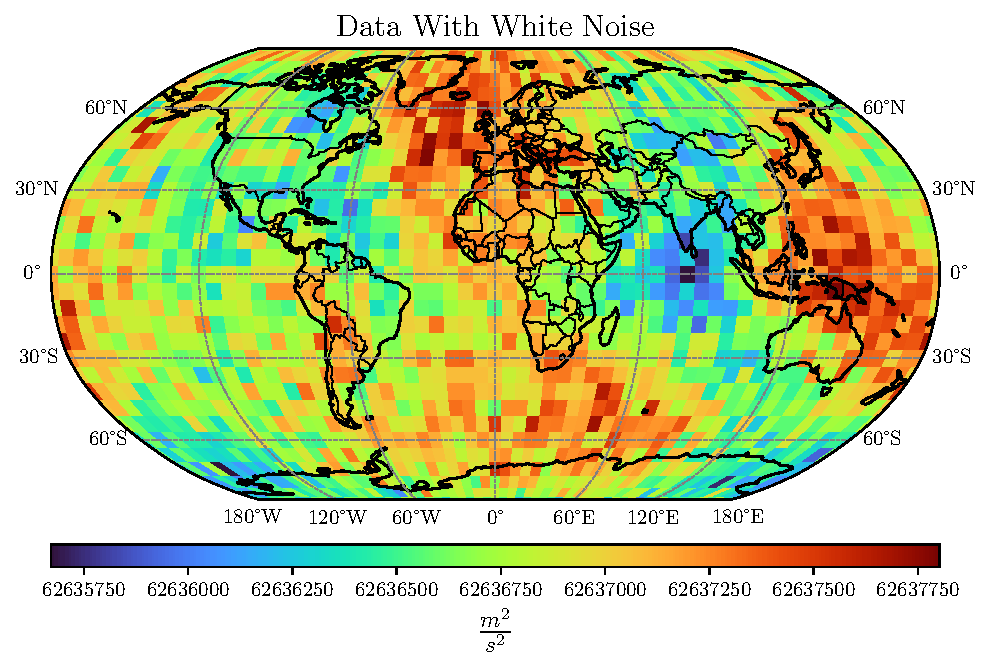
\includegraphics[height=6cm]{../Outputs/Plots/DataWithNoise.pdf}
		\caption{Input data after adding white noise with standard deviation of $200 \frac{m^2}{s^2}$.}
		\label{fig:DataWithNoise}
	\end{figure}
	
	\begin{table}[h!]
		\centering
		\caption{Results of interpolation using Abel-Poisson kernel and added white-noise (units of norm and mean values are $\frac{m^2}{s^2}$).}
		\vspace{0.2cm}
		\renewcommand{\arraystretch}{2}
		\begin{tabular}{c|c|c|c|c|c}
			\textbf{Method} & Cholesky & TSVD & GCV (FOT) & L-Curve (FOT) & VCE (FOT) \\
			\hline 
			\makecell{\textbf{Regularization} \\ \textbf{Parameter}} & --- & 145 & $3.50*10^{-6}$ & $5.33*10^{-4}$ & $2.03*10^{-7}$ \\
			\hline 
			\textit{\textbf{h}} & 0.065 & 0.381 & 0.121 & 0.201 & 0.173 \\
			\hline
			\textbf{Mean of Error} & \textcolor{blue}{0.1131} & 1.1173 & 4.1071 & 13.5542 & -3.1657 \\
			\hline 
			\textbf{Norm of Errors} & 5840.2691 & \textcolor{blue}{5735.7724} & 8289.586 & 21767.4379 & 6836.7964 \\
		\end{tabular}
		\label{tab:wn_Abel-Poisson_Results}
	\end{table}
	
	
	\begin{figure}[h!]
		\centering
		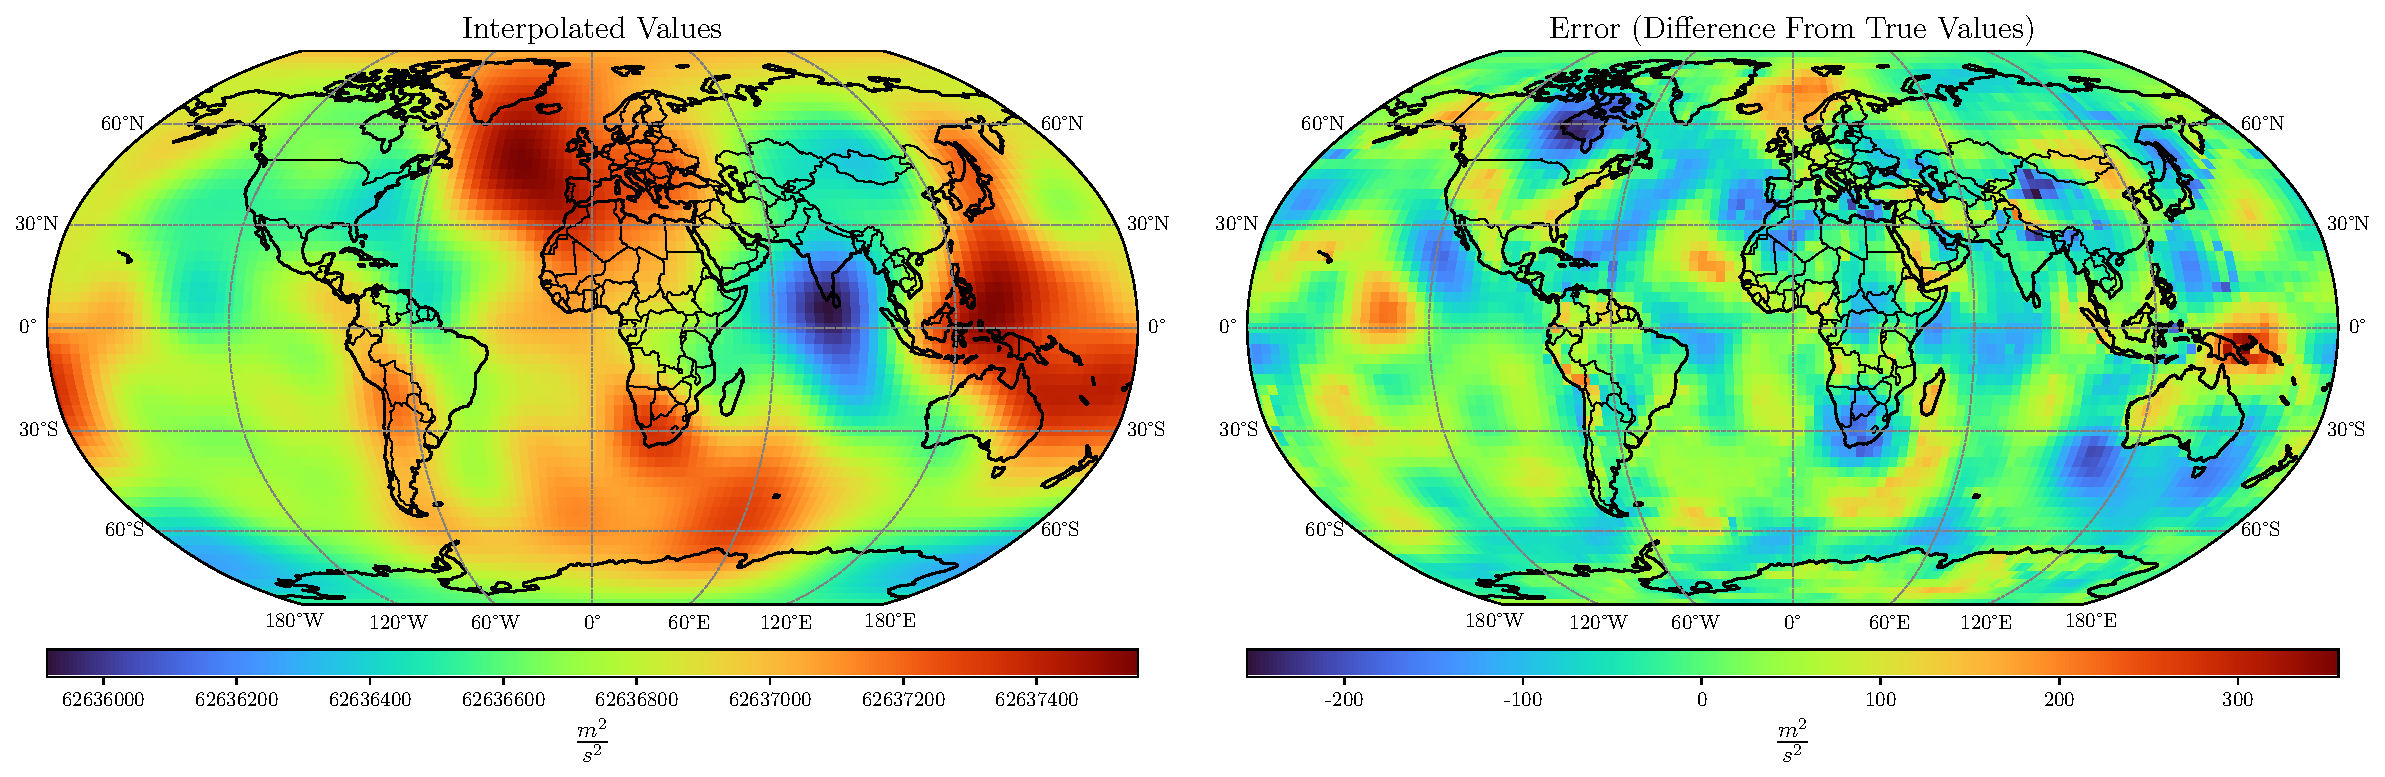
\includegraphics[width=16cm]{../Outputs/Plots/Plot_wn_Abel-Poisson_Cholesky.pdf}
		\caption{Results of Logarithmic kernel with Cholesky decomposition and added white-noise.}
		\label{fig:wn_Abel-Poisson_Chol}
	\end{figure}
	
	\begin{figure}[h!]
		\centering
		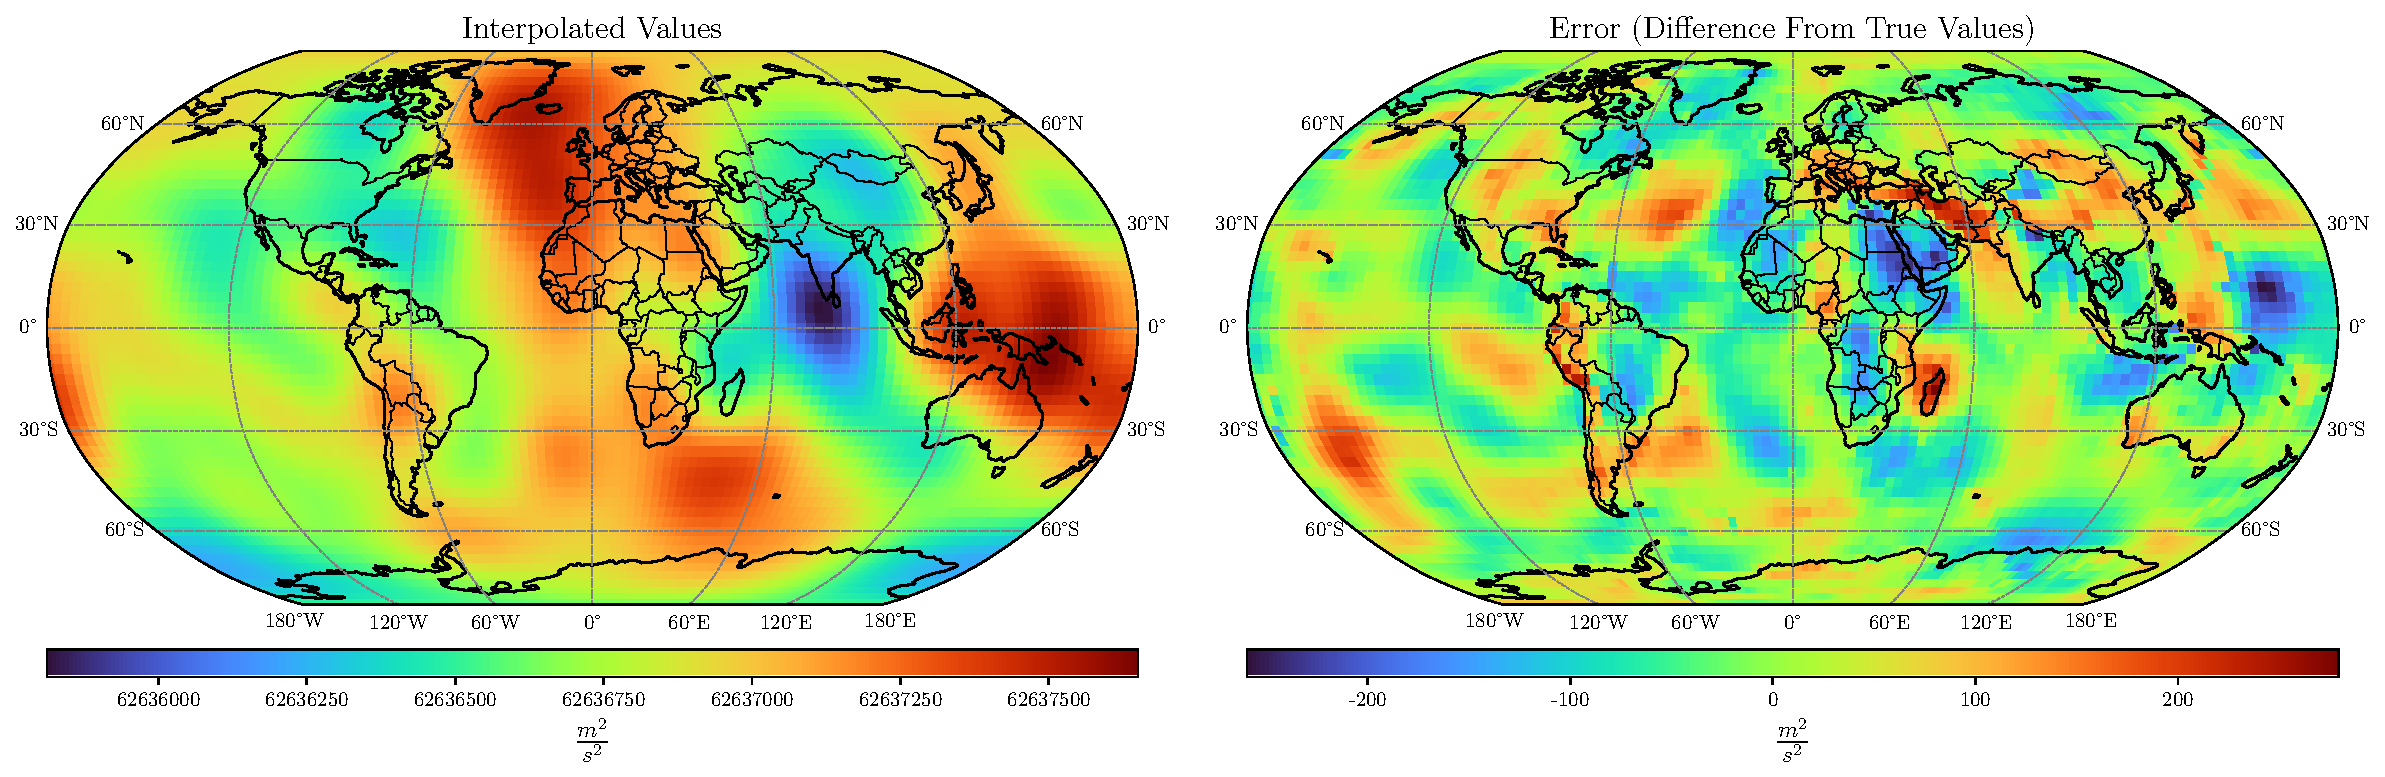
\includegraphics[width=16cm]{../Outputs/Plots/Plot_wn_Abel-Poisson_TSVD.pdf}
		\caption{Results of Logarithmic kernel with TSVD method and added white-noise.}
		\label{fig:wn_Abel-Poisson_TSVD}
	\end{figure}
	
	
	\begin{figure}[h!]
		\centering
		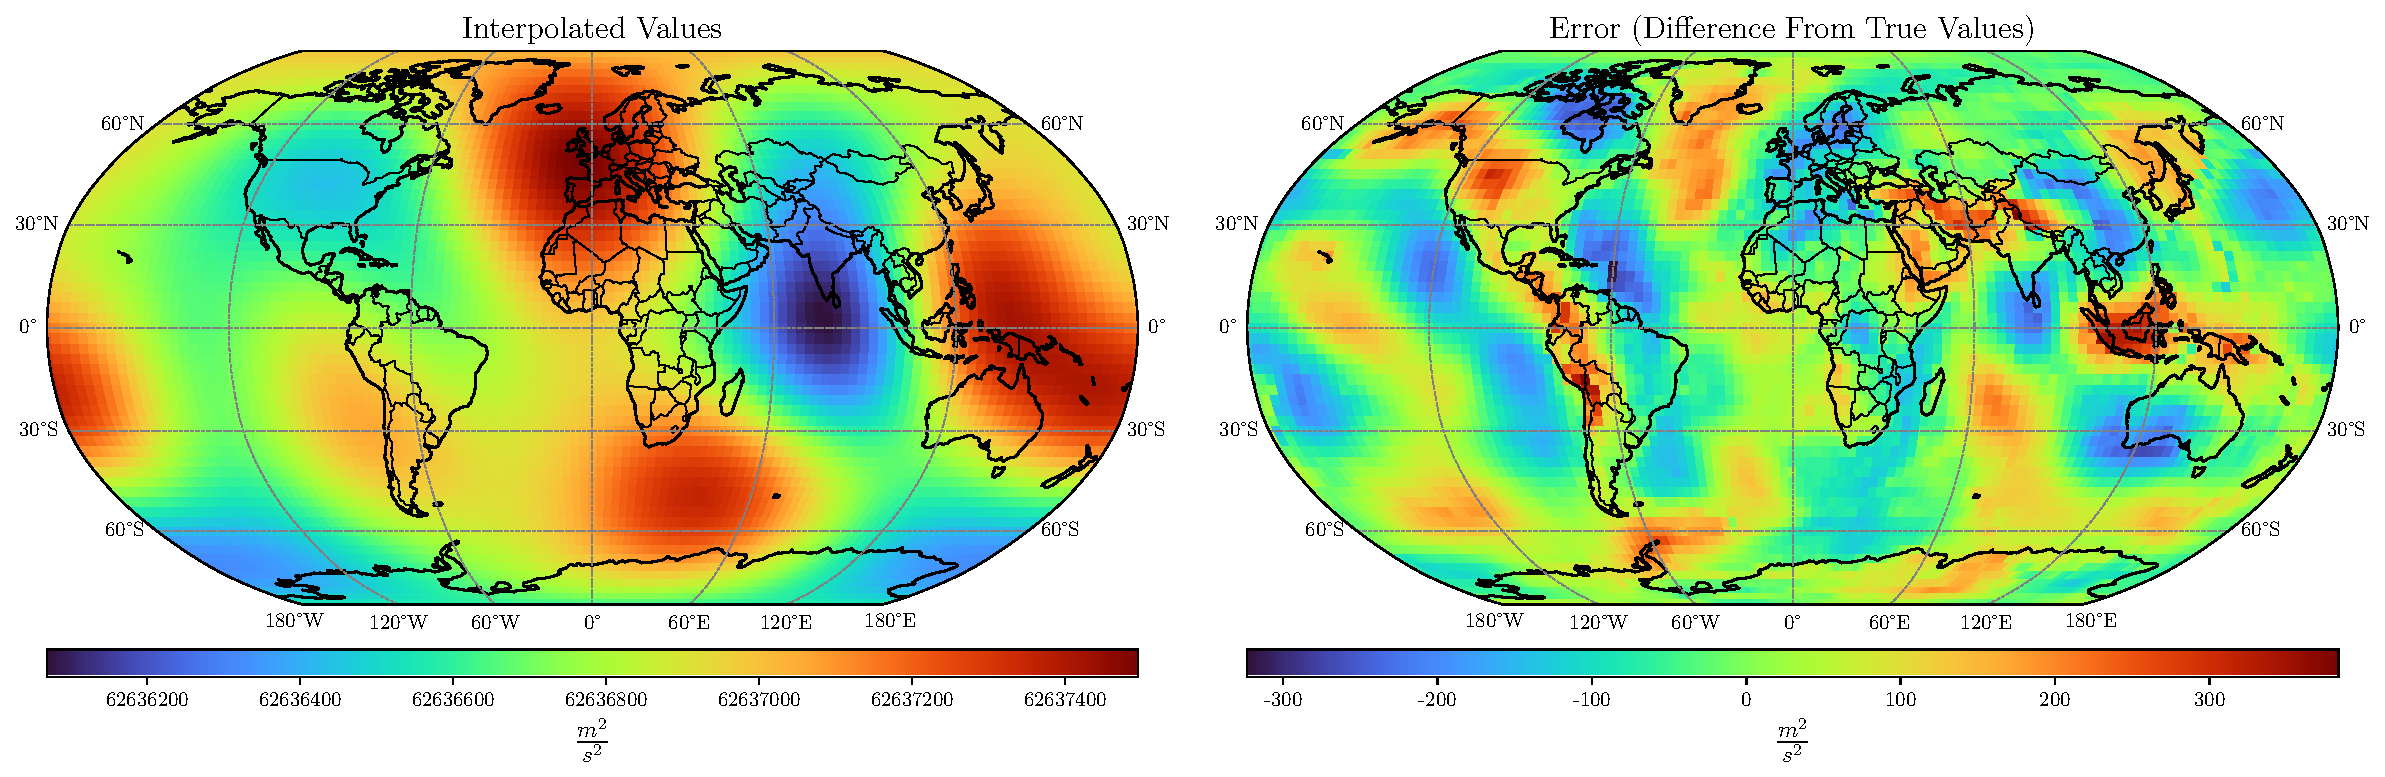
\includegraphics[width=16cm]{../Outputs/Plots/Plot_wn_Abel-Poisson_GCV.pdf}
		\caption{Results of Logarithmic kernel with GCV (FOT) method and added white-noise.}
		\label{fig:wn_Abel-Poisson_GCV}
	\end{figure}
	
	\begin{figure}[h!]
		\centering
		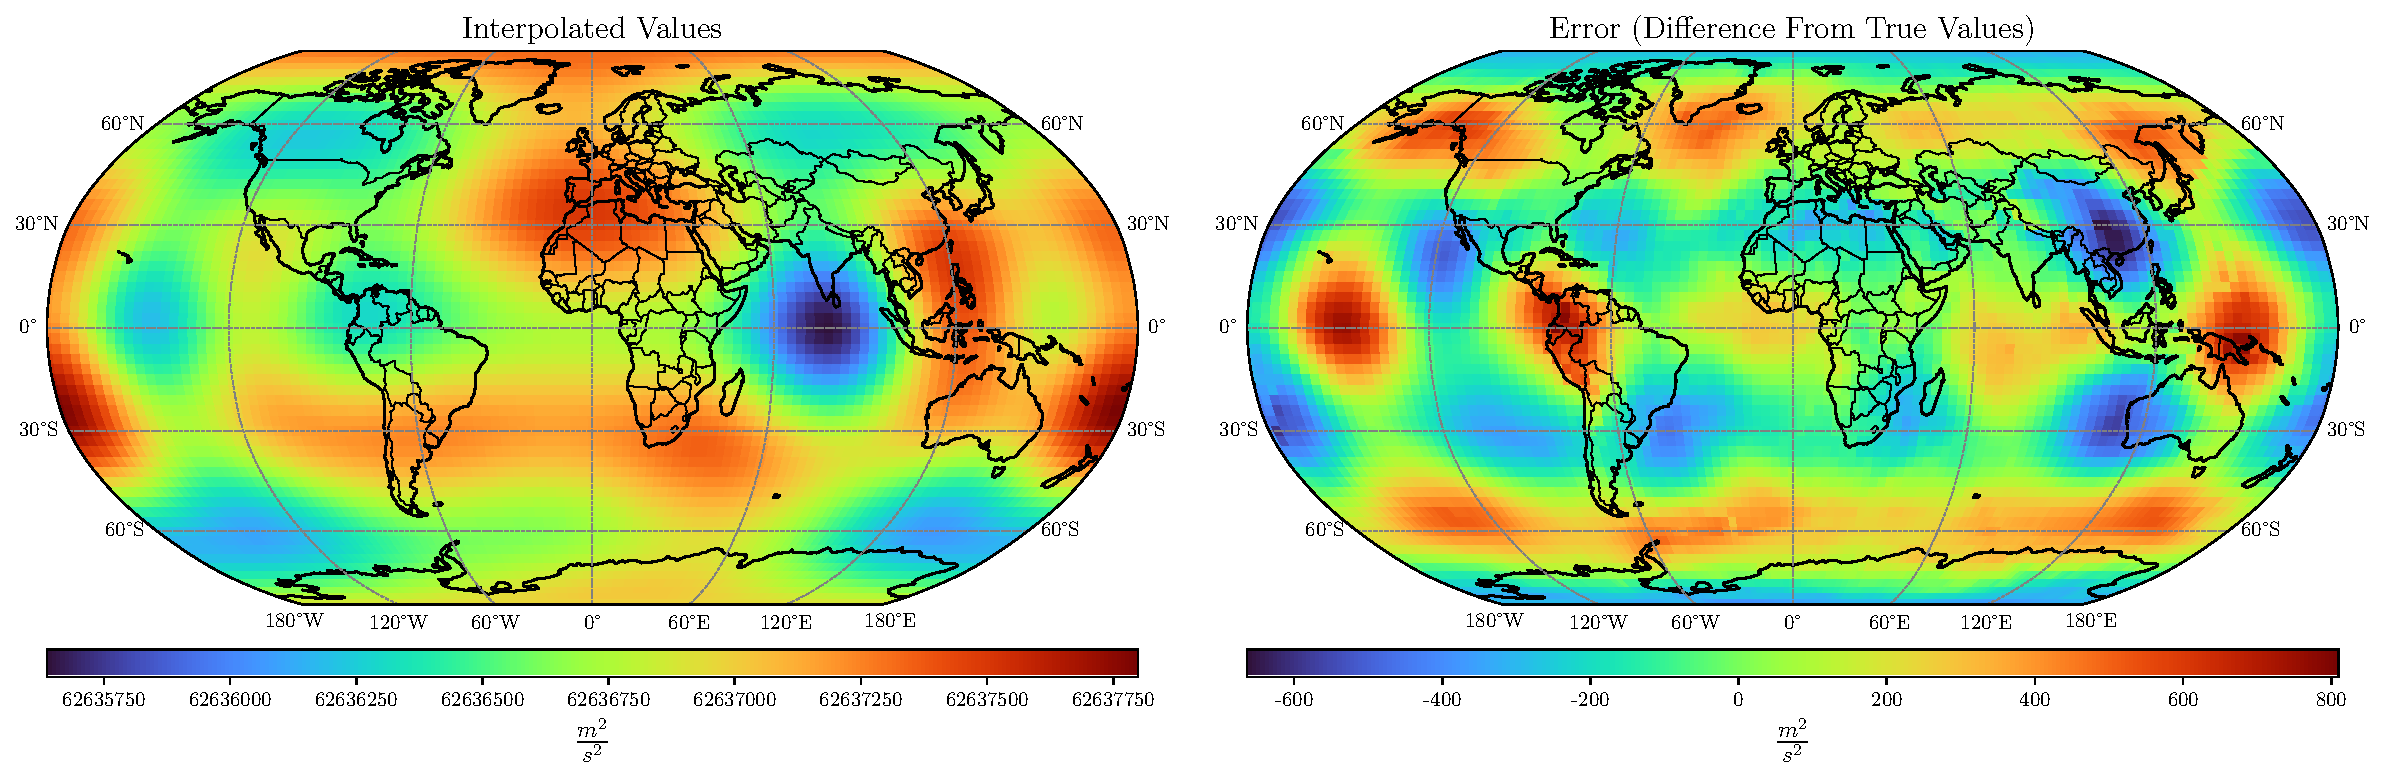
\includegraphics[width=16cm]{../Outputs/Plots/Plot_wn_Abel-Poisson_L-Curve.pdf}
		\caption{Results of Logarithmic kernel with L-Curve (FOT) method and added white-noise.}
		\label{fig:wn_Abel-Poisson_L-Curve}
	\end{figure}
	
	\clearpage
	
	\begin{figure}[h!]
		\centering
		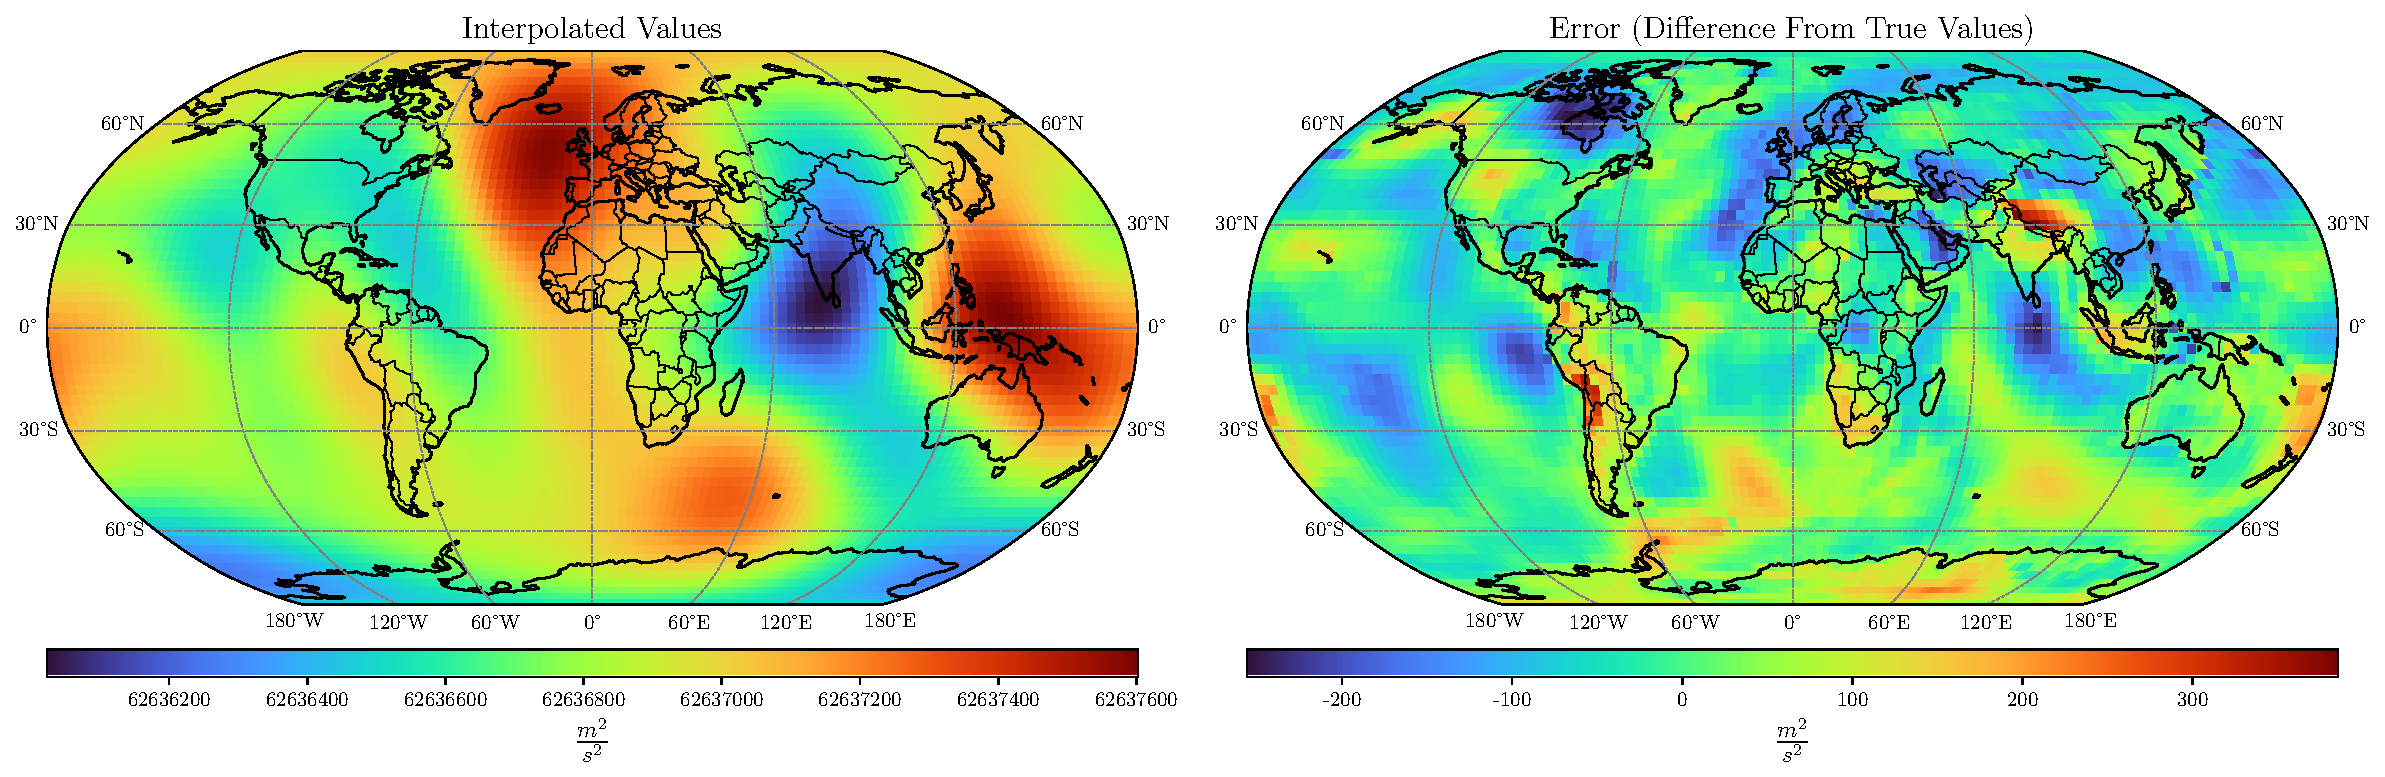
\includegraphics[width=16cm]{../Outputs/Plots/Plot_wn_Abel-Poisson_VCE.pdf}
		\caption{Results of Logarithmic kernel with VCE (FOT) method and added white-noise.}
		\label{fig:wn_Abel-Poisson_VCE}
	\end{figure}
	
	\section{Appendix}
	
	As mentioned before, for determining the value of $h$ in each kernel, a simple 3-step cross-validation method was implemented. As an example the norm mentioned in equation \ref{eq:CV} for different values of $h$ using TSVD method and three kernels are shown in figures \ref{fig:CV_Abel-Poisson_TSVD} to \ref{fig:CV_Logarithmic_TSVD}.
	
	\begin{figure}[h!]
		\centering
		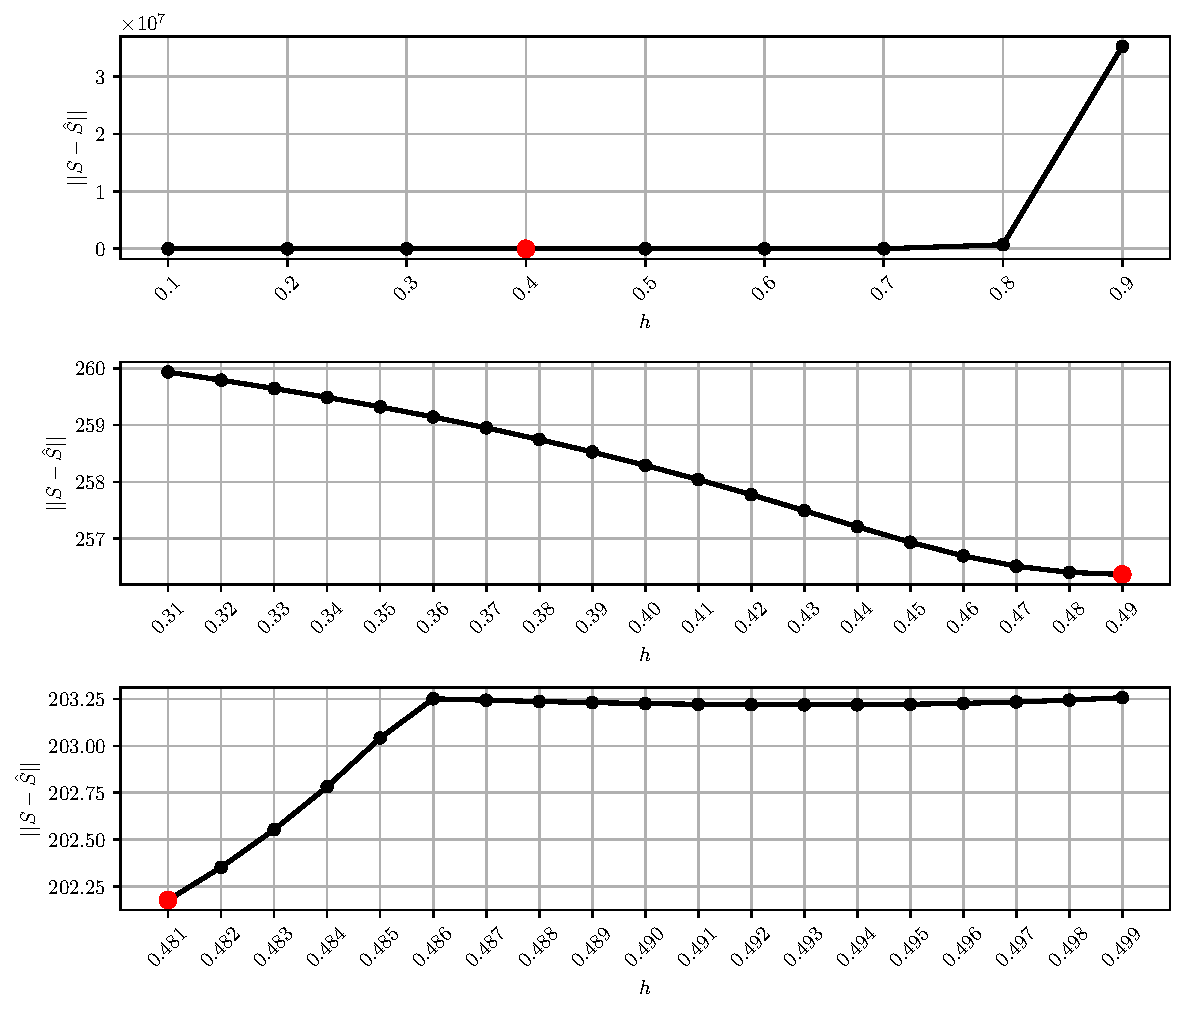
\includegraphics[height=9cm]{../Outputs/Plots/CV_Abel-Poisson_TSVD.pdf}
		\caption{Results of cross-validation method used for determining $h$ using Abel-Poisson kernel with TSVD method.}
		\label{fig:CV_Abel-Poisson_TSVD}
	\end{figure}
	
	\begin{figure}[h!]
		\centering
		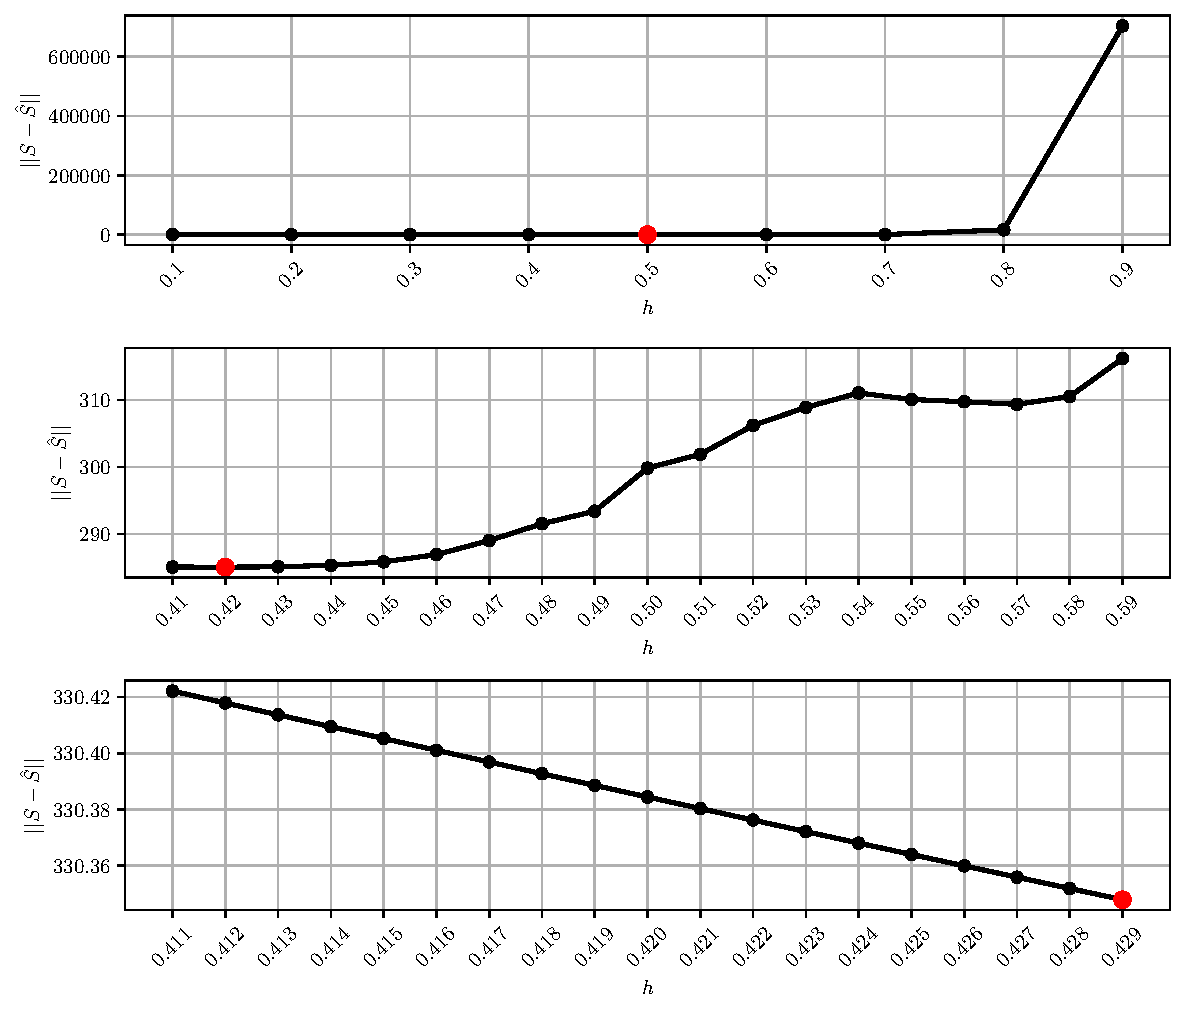
\includegraphics[height=9cm]{../Outputs/Plots/CV_Singularity_TSVD.pdf}
		\caption{Results of cross-validation method used for determining $h$ using Singularity kernel with TSVD method.}
		\label{fig:CV_Singularity_TSVD}
	\end{figure}
	
	\begin{figure}[h!]
		\centering
		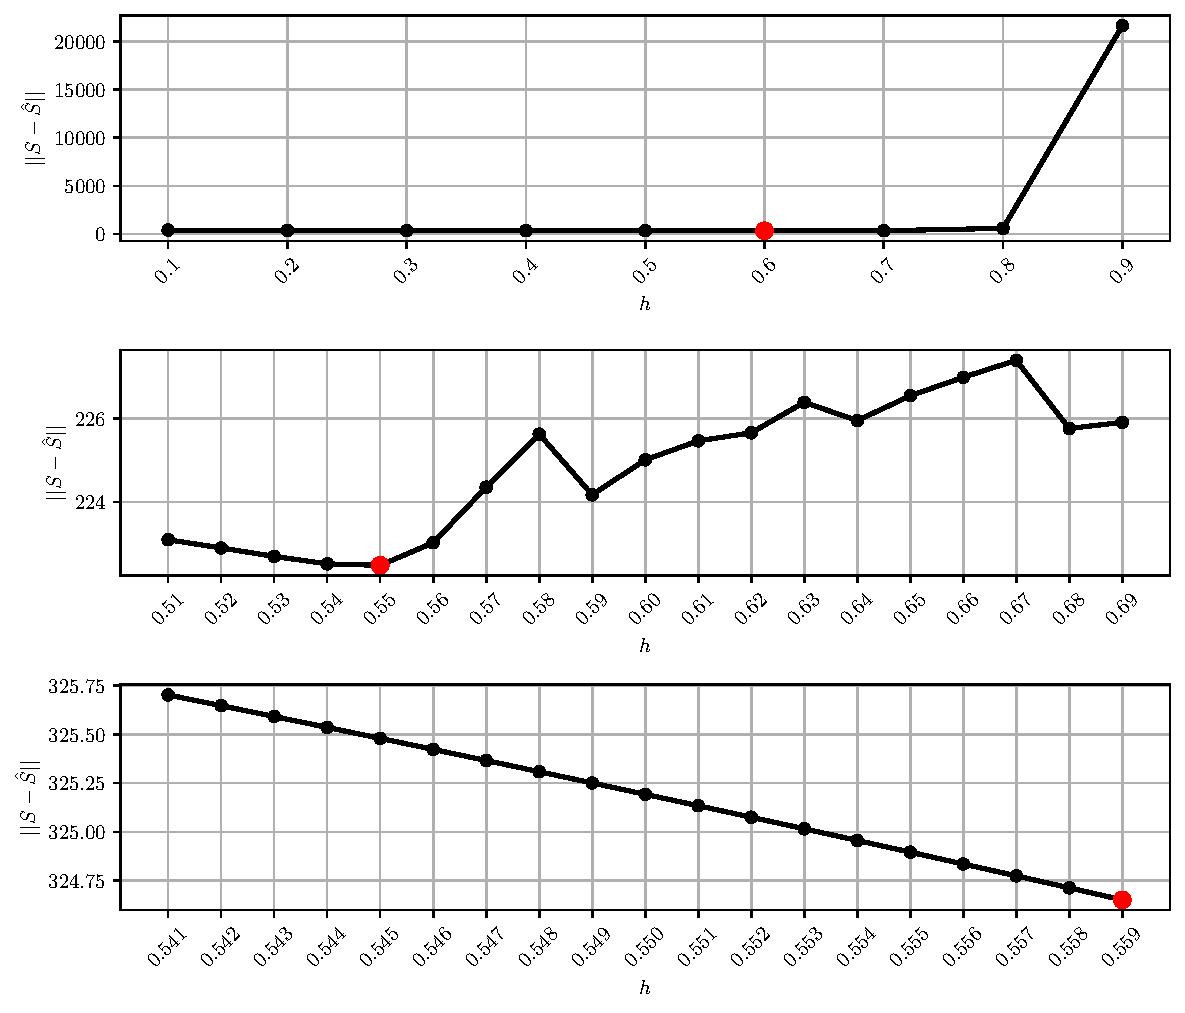
\includegraphics[height=9cm]{../Outputs/Plots/CV_Logarithmic_TSVD.pdf}
		\caption{Results of cross-validation method used for determining $h$ using Logarithmic kernel with TSVD method.}
		\label{fig:CV_Logarithmic_TSVD}
	\end{figure}
	
	\clearpage
	
	

\end{document}


